\documentclass[12pt]{article}
\usepackage[utf8]{inputenc}
\usepackage{graphicx}
\usepackage{parskip} 
\usepackage[nottoc]{tocbibind}
\graphicspath{ {images/} }
\title{Text classification using the semi-supervised methods}
\author{Michał Filek}
\date{June 2020}


\usepackage{natbib}
\usepackage{breakcites} % Do Not let citations break out of the text frame
\usepackage{microtype} % Get rid of some frame busts automatically
\usepackage{hyperref} 
\usepackage{booktabs}
\usepackage{float}
\usepackage[export]{adjustbox}
\usepackage{subcaption}
\usepackage{wrapfig}
\usepackage{amsmath}
\usepackage{nccmath}
\usepackage{fancyref}
% Note: if microtype causes error on ubuntu, run
% sudo apt-get install cm-super

\pdfobjcompresslevel=0

\usepackage{zref-abspage}

\setcounter{secnumdepth}{3} % Number subsubsections, because we reference them,
% so the reader needs numbers to find the correct place.

\usepackage[vcentering,dvips]{geometry}
\geometry{papersize={7in,9in},bottom=3pc,top=5pc,left=5pc,right=5pc,bmargin=4.5pc,footskip=18pt,headsep=25pt}

%%% Packages %%%
\usepackage{epsfig}
\usepackage{subfigure}
\usepackage[utf8]{inputenc}

% Needed for some foreign characters
\usepackage[T1]{fontenc}

\usepackage{amsmath}
\usepackage{subfigure}
\usepackage{amsfonts}
\usepackage{amsthm}
\usepackage{multirow}
\usepackage{colortbl}
\usepackage{booktabs}
% This allows us to cite chapters by name, which was useful for making the
% acknowledgements page
\usepackage{nameref}
% Make sure there is a space between the subsection number and subsection title
% in the table of contents.
% If we do not do this we end up with 2 digit subsection numbers colliding with
% the title.
% See https://tex.stackexchange.com/questions/7853/toc-text-numbers-alignment/7856#7856?newreg=d2632892dd0345f388619f12fa794b11
\usepackage[tocindentauto]{tocstyle}
\usetocstyle{standard}

\usepackage{bm}


\usepackage{float}
\newcommand{\boldindex}[1]{\textbf{\hyperpage{#1}}}
\usepackage{makeidx}\makeindex
% Make bibliography and index appear in table of contents
\usepackage[nottoc]{tocbibind}
% Using the caption package allows us to support captions that contain "itemize" environments.
% The font=small option makes the text of captions smaller than the main text.
\usepackage[font=small]{caption}

% Used to change header sizes
\usepackage{fancyhdr}


\theoremstyle{definition}
\newtheorem{example}{Example}[section]

% Define the P table cell environment
% It is the same as p, but centers the text horizontally
\usepackage{array}
\newcolumntype{P}[1]{>{\centering\arraybackslash}p{#1}}

% Rebuild the book document class's headers from scratch, but with different font size
% (this is for MIT Press style)
% Source: http://texblog.org/2012/10/09/changing-the-font-size-in-fancyhdr/
\newcommand{\changefont}{% 1st arg to fontsize is font size. 2nd arg is the baseline skip. both in points.
    \fontsize{9}{11}\selectfont
}
\DeclareMathOperator*{\argmax}{arg\!max}   % Jan Hlavacek
\DeclareMathOperator*{\argmin}{\arg\,min}
\fancyhf{}
%\fancyhead[LE,RO]{\changefont \slshape \rightmark} %section
\fancyfoot[C]{\changefont \thepage} %footer
\pagestyle{fancy}
%%%%% NEW MATH DEFINITIONS %%%%%

% Mark sections of captions for referring to divisions of figures
\newcommand{\figleft}{{\em (Left)}}
\newcommand{\figcenter}{{\em (Center)}}
\newcommand{\figright}{{\em (Right)}}
\newcommand{\figtop}{{\em (Top)}}
\newcommand{\figbottom}{{\em (Bottom)}}
\newcommand{\captiona}{{\em (a)}}
\newcommand{\captionb}{{\em (b)}}
\newcommand{\captionc}{{\em (c)}}
\newcommand{\captiond}{{\em (d)}}

% Highlight a newly defined term
\newcommand{\newterm}[1]{{\bf #1}}


% Figure reference, lower-case.
\def\figref#1{figure~\ref{#1}}
% Figure reference, capital. For start of sentence
\def\Figref#1{Figure~\ref{#1}}
\def\twofigref#1#2{figures \ref{#1} and \ref{#2}}
\def\quadfigref#1#2#3#4{figures \ref{#1}, \ref{#2}, \ref{#3} and \ref{#4}}
% Section reference, lower-case.
\def\secref#1{section~\ref{#1}}
% Section reference, capital.
\def\Secref#1{Section~\ref{#1}}
% Reference to two sections.
\def\twosecrefs#1#2{sections \ref{#1} and \ref{#2}}
% Reference to three sections.
\def\secrefs#1#2#3{sections \ref{#1}, \ref{#2} and \ref{#3}}
% Reference to an equation, lower-case.
\def\eqref#1{equation~\ref{#1}}
% Reference to an equation, upper case
\def\Eqref#1{Equation~\ref{#1}}
% A raw reference to an equation---avoid using if possible
\def\plaineqref#1{\ref{#1}}
% Reference to a chapter, lower-case.
\def\chapref#1{chapter~\ref{#1}}
% Reference to an equation, upper case.
\def\Chapref#1{Chapter~\ref{#1}}
% Reference to a range of chapters
\def\rangechapref#1#2{chapters\ref{#1}--\ref{#2}}
% Reference to an algorithm, lower-case.
\def\algref#1{algorithm~\ref{#1}}
% Reference to an algorithm, upper case.
\def\Algref#1{Algorithm~\ref{#1}}
\def\twoalgref#1#2{algorithms \ref{#1} and \ref{#2}}
\def\Twoalgref#1#2{Algorithms \ref{#1} and \ref{#2}}
% Reference to a part, lower case
\def\partref#1{part~\ref{#1}}
% Reference to a part, upper case
\def\Partref#1{Part~\ref{#1}}
\def\twopartref#1#2{parts \ref{#1} and \ref{#2}}

\def\ceil#1{\lceil #1 \rceil}
\def\floor#1{\lfloor #1 \rfloor}
\def\1{\bm{1}}
\newcommand{\train}{\mathcal{D}}
\newcommand{\valid}{\mathcal{D_{\mathrm{valid}}}}
\newcommand{\test}{\mathcal{D_{\mathrm{test}}}}

\def\eps{{\epsilon}}


% Random variables
\def\reta{{\textnormal{$\eta$}}}
\def\ra{{\textnormal{a}}}
\def\rb{{\textnormal{b}}}
\def\rc{{\textnormal{c}}}
\def\rd{{\textnormal{d}}}
\def\re{{\textnormal{e}}}
\def\rf{{\textnormal{f}}}
\def\rg{{\textnormal{g}}}
\def\rh{{\textnormal{h}}}
\def\ri{{\textnormal{i}}}
\def\rj{{\textnormal{j}}}
\def\rk{{\textnormal{k}}}
\def\rl{{\textnormal{l}}}
% rm is already a command, just don't name any random variables m
\def\rn{{\textnormal{n}}}
\def\ro{{\textnormal{o}}}
\def\rp{{\textnormal{p}}}
\def\rq{{\textnormal{q}}}
\def\rr{{\textnormal{r}}}
\def\rs{{\textnormal{s}}}
\def\rt{{\textnormal{t}}}
\def\ru{{\textnormal{u}}}
\def\rv{{\textnormal{v}}}
\def\rw{{\textnormal{w}}}
\def\rx{{\textnormal{x}}}
\def\ry{{\textnormal{y}}}
\def\rz{{\textnormal{z}}}

% Random vectors
\def\rvepsilon{{\mathbf{\epsilon}}}
\def\rvtheta{{\mathbf{\theta}}}
\def\rva{{\mathbf{a}}}
\def\rvb{{\mathbf{b}}}
\def\rvc{{\mathbf{c}}}
\def\rvd{{\mathbf{d}}}
\def\rve{{\mathbf{e}}}
\def\rvf{{\mathbf{f}}}
\def\rvg{{\mathbf{g}}}
\def\rvh{{\mathbf{h}}}
\def\rvu{{\mathbf{i}}}
\def\rvj{{\mathbf{j}}}
\def\rvk{{\mathbf{k}}}
\def\rvl{{\mathbf{l}}}
\def\rvm{{\mathbf{m}}}
\def\rvn{{\mathbf{n}}}
\def\rvo{{\mathbf{o}}}
\def\rvp{{\mathbf{p}}}
\def\rvq{{\mathbf{q}}}
\def\rvr{{\mathbf{r}}}
\def\rvs{{\mathbf{s}}}
\def\rvt{{\mathbf{t}}}
\def\rvu{{\mathbf{u}}}
\def\rvv{{\mathbf{v}}}
\def\rvw{{\mathbf{w}}}
\def\rvx{{\mathbf{x}}}
\def\rvy{{\mathbf{y}}}
\def\rvz{{\mathbf{z}}}

% Elements of random vectors
\def\erva{{\textnormal{a}}}
\def\ervb{{\textnormal{b}}}
\def\ervc{{\textnormal{c}}}
\def\ervd{{\textnormal{d}}}
\def\erve{{\textnormal{e}}}
\def\ervf{{\textnormal{f}}}
\def\ervg{{\textnormal{g}}}
\def\ervh{{\textnormal{h}}}
\def\ervi{{\textnormal{i}}}
\def\ervj{{\textnormal{j}}}
\def\ervk{{\textnormal{k}}}
\def\ervl{{\textnormal{l}}}
\def\ervm{{\textnormal{m}}}
\def\ervn{{\textnormal{n}}}
\def\ervo{{\textnormal{o}}}
\def\ervp{{\textnormal{p}}}
\def\ervq{{\textnormal{q}}}
\def\ervr{{\textnormal{r}}}
\def\ervs{{\textnormal{s}}}
\def\ervt{{\textnormal{t}}}
\def\ervu{{\textnormal{u}}}
\def\ervv{{\textnormal{v}}}
\def\ervw{{\textnormal{w}}}
\def\ervx{{\textnormal{x}}}
\def\ervy{{\textnormal{y}}}
\def\ervz{{\textnormal{z}}}

% Random matrices
\def\rmA{{\mathbf{A}}}
\def\rmB{{\mathbf{B}}}
\def\rmC{{\mathbf{C}}}
\def\rmD{{\mathbf{D}}}
\def\rmE{{\mathbf{E}}}
\def\rmF{{\mathbf{F}}}
\def\rmG{{\mathbf{G}}}
\def\rmH{{\mathbf{H}}}
\def\rmI{{\mathbf{I}}}
\def\rmJ{{\mathbf{J}}}
\def\rmK{{\mathbf{K}}}
\def\rmL{{\mathbf{L}}}
\def\rmM{{\mathbf{M}}}
\def\rmN{{\mathbf{N}}}
\def\rmO{{\mathbf{O}}}
\def\rmP{{\mathbf{P}}}
\def\rmQ{{\mathbf{Q}}}
\def\rmR{{\mathbf{R}}}
\def\rmS{{\mathbf{S}}}
\def\rmT{{\mathbf{T}}}
\def\rmU{{\mathbf{U}}}
\def\rmV{{\mathbf{V}}}
\def\rmW{{\mathbf{W}}}
\def\rmX{{\mathbf{X}}}
\def\rmY{{\mathbf{Y}}}
\def\rmZ{{\mathbf{Z}}}

% Elements of random matrices
\def\ermA{{\textnormal{A}}}
\def\ermB{{\textnormal{B}}}
\def\ermC{{\textnormal{C}}}
\def\ermD{{\textnormal{D}}}
\def\ermE{{\textnormal{E}}}
\def\ermF{{\textnormal{F}}}
\def\ermG{{\textnormal{G}}}
\def\ermH{{\textnormal{H}}}
\def\ermI{{\textnormal{I}}}
\def\ermJ{{\textnormal{J}}}
\def\ermK{{\textnormal{K}}}
\def\ermL{{\textnormal{L}}}
\def\ermM{{\textnormal{M}}}
\def\ermN{{\textnormal{N}}}
\def\ermO{{\textnormal{O}}}
\def\ermP{{\textnormal{P}}}
\def\ermQ{{\textnormal{Q}}}
\def\ermR{{\textnormal{R}}}
\def\ermS{{\textnormal{S}}}
\def\ermT{{\textnormal{T}}}
\def\ermU{{\textnormal{U}}}
\def\ermV{{\textnormal{V}}}
\def\ermW{{\textnormal{W}}}
\def\ermX{{\textnormal{X}}}
\def\ermY{{\textnormal{Y}}}
\def\ermZ{{\textnormal{Z}}}

% Vectors
\def\vzero{{\bm{0}}}
\def\vone{{\bm{1}}}
\def\vmu{{\bm{\mu}}}
\def\vtheta{{\bm{\theta}}}
\def\va{{\bm{a}}}
\def\vb{{\bm{b}}}
\def\vc{{\bm{c}}}
\def\vd{{\bm{d}}}
\def\ve{{\bm{e}}}
\def\vf{{\bm{f}}}
\def\vg{{\bm{g}}}
\def\vh{{\bm{h}}}
\def\vi{{\bm{i}}}
\def\vj{{\bm{j}}}
\def\vk{{\bm{k}}}
\def\vl{{\bm{l}}}
\def\vm{{\bm{m}}}
\def\vn{{\bm{n}}}
\def\vo{{\bm{o}}}
\def\vp{{\bm{p}}}
\def\vq{{\bm{q}}}
\def\vr{{\bm{r}}}
\def\vs{{\bm{s}}}
\def\vt{{\bm{t}}}
\def\vu{{\bm{u}}}
\def\vv{{\bm{v}}}
\def\vw{{\bm{w}}}
\def\vx{{\bm{x}}}
\def\vy{{\bm{y}}}
\def\vz{{\bm{z}}}

% Elements of vectors
\def\evalpha{{\alpha}}
\def\evbeta{{\beta}}
\def\evepsilon{{\epsilon}}
\def\evlambda{{\lambda}}
\def\evomega{{\omega}}
\def\evmu{{\mu}}
\def\evpsi{{\psi}}
\def\evsigma{{\sigma}}
\def\evtheta{{\theta}}
\def\eva{{a}}
\def\evb{{b}}
\def\evc{{c}}
\def\evd{{d}}
\def\eve{{e}}
\def\evf{{f}}
\def\evg{{g}}
\def\evh{{h}}
\def\evi{{i}}
\def\evj{{j}}
\def\evk{{k}}
\def\evl{{l}}
\def\evm{{m}}
\def\evn{{n}}
\def\evo{{o}}
\def\evp{{p}}
\def\evq{{q}}
\def\evr{{r}}
\def\evs{{s}}
\def\evt{{t}}
\def\evu{{u}}
\def\evv{{v}}
\def\evw{{w}}
\def\evx{{x}}
\def\evy{{y}}
\def\evz{{z}}

% Matrix
\def\mA{{\bm{A}}}
\def\mB{{\bm{B}}}
\def\mC{{\bm{C}}}
\def\mD{{\bm{D}}}
\def\mE{{\bm{E}}}
\def\mF{{\bm{F}}}
\def\mG{{\bm{G}}}
\def\mH{{\bm{H}}}
\def\mI{{\bm{I}}}
\def\mJ{{\bm{J}}}
\def\mK{{\bm{K}}}
\def\mL{{\bm{L}}}
\def\mM{{\bm{M}}}
\def\mN{{\bm{N}}}
\def\mO{{\bm{O}}}
\def\mP{{\bm{P}}}
\def\mQ{{\bm{Q}}}
\def\mR{{\bm{R}}}
\def\mS{{\bm{S}}}
\def\mT{{\bm{T}}}
\def\mU{{\bm{U}}}
\def\mV{{\bm{V}}}
\def\mW{{\bm{W}}}
\def\mX{{\bm{X}}}
\def\mY{{\bm{Y}}}
\def\mZ{{\bm{Z}}}
\def\mBeta{{\bm{\beta}}}
\def\mPhi{{\bm{\Phi}}}
\def\mLambda{{\bm{\Lambda}}}
\def\mSigma{{\bm{\Sigma}}}

% Tensor
\DeclareMathAlphabet{\mathsfit}{\encodingdefault}{\sfdefault}{m}{sl}
\SetMathAlphabet{\mathsfit}{bold}{\encodingdefault}{\sfdefault}{bx}{n}
\newcommand{\tens}[1]{\bm{\mathsfit{#1}}}
\def\tA{{\tens{A}}}
\def\tB{{\tens{B}}}
\def\tC{{\tens{C}}}
\def\tD{{\tens{D}}}
\def\tE{{\tens{E}}}
\def\tF{{\tens{F}}}
\def\tG{{\tens{G}}}
\def\tH{{\tens{H}}}
\def\tI{{\tens{I}}}
\def\tJ{{\tens{J}}}
\def\tK{{\tens{K}}}
\def\tL{{\tens{L}}}
\def\tM{{\tens{M}}}
\def\tN{{\tens{N}}}
\def\tO{{\tens{O}}}
\def\tP{{\tens{P}}}
\def\tQ{{\tens{Q}}}
\def\tR{{\tens{R}}}
\def\tS{{\tens{S}}}
\def\tT{{\tens{T}}}
\def\tU{{\tens{U}}}
\def\tV{{\tens{V}}}
\def\tW{{\tens{W}}}
\def\tX{{\tens{X}}}
\def\tY{{\tens{Y}}}
\def\tZ{{\tens{Z}}}


% Graph
\def\gA{{\mathcal{A}}}
\def\gB{{\mathcal{B}}}
\def\gC{{\mathcal{C}}}
\def\gD{{\mathcal{D}}}
\def\gE{{\mathcal{E}}}
\def\gF{{\mathcal{F}}}
\def\gG{{\mathcal{G}}}
\def\gH{{\mathcal{H}}}
\def\gI{{\mathcal{I}}}
\def\gJ{{\mathcal{J}}}
\def\gK{{\mathcal{K}}}
\def\gL{{\mathcal{L}}}
\def\gM{{\mathcal{M}}}
\def\gN{{\mathcal{N}}}
\def\gO{{\mathcal{O}}}
\def\gP{{\mathcal{P}}}
\def\gQ{{\mathcal{Q}}}
\def\gR{{\mathcal{R}}}
\def\gS{{\mathcal{S}}}
\def\gT{{\mathcal{T}}}
\def\gU{{\mathcal{U}}}
\def\gV{{\mathcal{V}}}
\def\gW{{\mathcal{W}}}
\def\gX{{\mathcal{X}}}
\def\gY{{\mathcal{Y}}}
\def\gZ{{\mathcal{Z}}}

% Sets
\def\sA{{\mathbb{A}}}
\def\sB{{\mathbb{B}}}
\def\sC{{\mathbb{C}}}
\def\sD{{\mathbb{D}}}
% Don't use a set called E, because this would be the same as our symbol
% for expectation.
\def\sF{{\mathbb{F}}}
\def\sG{{\mathbb{G}}}
\def\sH{{\mathbb{H}}}
\def\sI{{\mathbb{I}}}
\def\sJ{{\mathbb{J}}}
\def\sK{{\mathbb{K}}}
\def\sL{{\mathbb{L}}}
\def\sM{{\mathbb{M}}}
\def\sN{{\mathbb{N}}}
\def\sO{{\mathbb{O}}}
\def\sP{{\mathbb{P}}}
\def\sQ{{\mathbb{Q}}}
\def\sR{{\mathbb{R}}}
\def\sS{{\mathbb{S}}}
\def\sT{{\mathbb{T}}}
\def\sU{{\mathbb{U}}}
\def\sV{{\mathbb{V}}}
\def\sW{{\mathbb{W}}}
\def\sX{{\mathbb{X}}}
\def\sY{{\mathbb{Y}}}
\def\sZ{{\mathbb{Z}}}

% Entries of a matrix
\def\emLambda{{\Lambda}}
\def\emA{{A}}
\def\emB{{B}}
\def\emC{{C}}
\def\emD{{D}}
\def\emE{{E}}
\def\emF{{F}}
\def\emG{{G}}
\def\emH{{H}}
\def\emI{{I}}
\def\emJ{{J}}
\def\emK{{K}}
\def\emL{{L}}
\def\emM{{M}}
\def\emN{{N}}
\def\emO{{O}}
\def\emP{{P}}
\def\emQ{{Q}}
\def\emR{{R}}
\def\emS{{S}}
\def\emT{{T}}
\def\emU{{U}}
\def\emV{{V}}
\def\emW{{W}}
\def\emX{{X}}
\def\emY{{Y}}
\def\emZ{{Z}}
\def\emSigma{{\Sigma}}

% entries of a tensor
% Same font as tensor, without \bm wrapper
\newcommand{\etens}[1]{\mathsfit{#1}}
\def\etLambda{{\etens{\Lambda}}}
\def\etA{{\etens{A}}}
\def\etB{{\etens{B}}}
\def\etC{{\etens{C}}}
\def\etD{{\etens{D}}}
\def\etE{{\etens{E}}}
\def\etF{{\etens{F}}}
\def\etG{{\etens{G}}}
\def\etH{{\etens{H}}}
\def\etI{{\etens{I}}}
\def\etJ{{\etens{J}}}
\def\etK{{\etens{K}}}
\def\etL{{\etens{L}}}
\def\etM{{\etens{M}}}
\def\etN{{\etens{N}}}
\def\etO{{\etens{O}}}
\def\etP{{\etens{P}}}
\def\etQ{{\etens{Q}}}
\def\etR{{\etens{R}}}
\def\etS{{\etens{S}}}
\def\etT{{\etens{T}}}
\def\etU{{\etens{U}}}
\def\etV{{\etens{V}}}
\def\etW{{\etens{W}}}
\def\etX{{\etens{X}}}
\def\etY{{\etens{Y}}}
\def\etZ{{\etens{Z}}}

% The true underlying data generating distribution
\newcommand{\pdata}{p_{\rm{data}}}
% The empirical distribution defined by the training set
\newcommand{\ptrain}{\hat{p}_{\rm{data}}}
\newcommand{\Ptrain}{\hat{P}_{\rm{data}}}
% The model distribution
\newcommand{\pmodel}{p_{\rm{model}}}
\newcommand{\Pmodel}{P_{\rm{model}}}
\newcommand{\ptildemodel}{\tilde{p}_{\rm{model}}}
% Stochastic autoencoder distributions
\newcommand{\pencode}{p_{\rm{encoder}}}
\newcommand{\pdecode}{p_{\rm{decoder}}}
\newcommand{\precons}{p_{\rm{reconstruct}}}

\newcommand{\laplace}{\mathrm{Laplace}} % Laplace distribution

\newcommand{\E}{\mathbb{E}}
\newcommand{\Ls}{\mathcal{L}}
\newcommand{\R}{\mathbb{R}}
\newcommand{\emp}{\tilde{p}}
\newcommand{\lr}{\alpha}
\newcommand{\reg}{\lambda}
\newcommand{\rect}{\mathrm{rectifier}}
\newcommand{\softmax}{\mathrm{softmax}}
\newcommand{\sigmoid}{\sigma}
\newcommand{\softplus}{\zeta}
\newcommand{\KL}{D_{\mathrm{KL}}}
\newcommand{\Var}{\mathrm{Var}}
\newcommand{\standarderror}{\mathrm{SE}}
\newcommand{\Cov}{\mathrm{Cov}}
% Wolfram Mathworld says $L^2$ is for function spaces and $\ell^2$ is for vectors
% But then they seem to use $L^2$ for vectors throughout the site, and so does
% wikipedia.
\newcommand{\normlzero}{L^0}
\newcommand{\normlone}{L^1}
\newcommand{\normltwo}{L^2}
\newcommand{\normlp}{L^p}
\newcommand{\normmax}{L^\infty}

\newcommand{\parents}{Pa} % See usage in notation.tex. Chosen to match Daphne's book.

\DeclareMathOperator*{\argmax}{arg\,max}
\DeclareMathOperator*{\argmin}{arg\,min}

\DeclareMathOperator{\sign}{sign}
\DeclareMathOperator{\Tr}{Tr}
\let\ab\allowbreak


% Make \[ \] math have equation numbers
\DeclareRobustCommand{\[}{\begin{equation}}
\DeclareRobustCommand{\]}{\end{equation}}

% Allow align environments to cross page boundaries.
% If we do not do this, we get weird gaps of several inches of white space
% before or after some long align environments.
\allowdisplaybreaks

\begin{document}

\setlength{\parskip}{0.25 \baselineskip}
\newlength{\figwidth}
\setlength{\figwidth}{26pc}
% Spacing between notation sections
\newlength{\notationgap}
\setlength{\notationgap}{1pc}
\setlength{\parindent}{4ex}
\thispagestyle{empty}
\begin{titlepage}
    \begin{center}

           \Large
	\textbf{Jagiellonian University}\vspace{0.2cm}\\ Faculty of Mathematics and Computer Science
               \vspace*{1cm}
               
         \vspace{3cm}
         \Large
          \textbf{Michał Filek}\\\vspace{0.5cm}
         \normalsize Album nr: 1157814\\
             \vspace{2cm}
        \Huge
        \textbf{Text classification using the semi-supervised methods }
      
        \vspace{1.5cm}
        \normalsize
        Master Thesis\\
        Field of study: Computer Science\\ \vspace{0.15cm}
        
        \vfill
        \vspace{2cm}
       \begin{minipage}{1\textwidth}
\begin{flushright}
Supervisor:\\
Dr Marek Śmieja\\
Institute of Computer Science and Computational Mathematics
\end{flushright}
\end{minipage}
        
        \vspace{2cm}
        \begin{center}
      Cracow 2020
        \end{center}
    \end{center}
\end{titlepage}

\newpage 
 \thispagestyle{empty}
\vspace{2.5cm}
\begin{flushleft}
\large \textbf{Author's statement}\vspace{0.6cm}\\
\end{flushleft}

\noindent Being aware of legal responsibility, I declare that this diploma thesis was written by myself and does not contain content obtained in a manner inconsistent with applicable regulations.\\

\noindent I also certify that the presented thesis has not been subject to procedures related to obtaining a professional title at a university..
\vspace{2cm}
\begin{center}
\begin{tabular}{lr}
................................~~~~~~~~~~~~~~~~~~~~~~~~~~~~~~~~~~~~~~&
.......................................... \\
{~~~~Cracow, date} & {Author's signature~~~~}
\end{tabular}
\end{center}
\vspace{5cm}
\begin{flushleft}
\large \textbf{Thesis supervisor's statement}
\end{flushleft}

\noindent I confirm that this work has been prepared under my supervision and is eligible to be presented in the procedure for granting the professional title.
\vspace{2cm}
\begin{center}
\begin{tabular}{lr}
................................~~~~~~~~~~~~~~~~~~~~~~~~~~~~~~~~~~~~~~&
............................................ \\
{~~~~Cracow, date} & {Thesis supervisor's signature~~}
\end{tabular}
\end{center}
\vfill
\vspace{2cm}
\vfill




% ABSTRACT
\begin{abstract}
The work is devoted to the issue of semi-supervised learning for the tasks of text classification. One of the aims  is to test the semi-supervised learning algorithm called FixMatch in the NLP domain. This method is considered to be state-of-the-art for problems of image classification with very few training labeled examples. In order to test FixMatch for text classification, it is necessary to create realistic augmentations, which will be proposed in the following work. In order to evaluate the FixMatch properly, two other popular SSL methods (VAT, Pseudo-Label) and supervised model, will be trained as comparative baselines. Another goal of the work is to check how the result on the test set are affected by training process and selection of hyperparameters using different ratio of the training and validation set sizes. The last goal will be to examine the quality of the chosen hyperparameter on small validation sets, also by checking the results of the SLL methods used with more labelled and unlabeled data. \par
 Results of conducted experiments for the FixMatch algorithm indicate that it was not possible to repeat in the text domain state-of-the-art scores from the computer vision domain. After observing the results of successful experiments with different SSL methods, a conclusion appears that the number of examples in the validation set should be slightly less or equal to the number of examples in the training set. For used SSL methods, the error on the test set is decreasing with training on an additional number of labeled data, while in the case of unlabeled data, there is no such relation.
\end{abstract}
\vspace{2cm}
\vspace{2cm}
\vspace{2cm}
\tableofcontents
\medskip

%\section{Notation}
\label{notation}

% Sometimes we have to include the following line to get this section
% included in the Table of Contents despite being a chapter*
This section provides a concise reference describing notation used throughout this
document.
If you are unfamiliar with any of the corresponding mathematical concepts,
\citet{dlbook} describe most of these ideas in
chapters 2--4.

\vspace{\notationgap}
% Need to use minipage to keep title of table on same page as table
\begin{minipage}{\textwidth}
% This is a hack to put a little title over the table
% We cannot use "\section*", etc., they appear in the table of contents.
% tocdepth does not work on this chapter.
\centerline{\bf Numbers and Arrays}
\bgroup
% The \arraystretch definition here increases the space between rows in the table,
% so that \displaystyle math has more vertical space.
\def\arraystretch{1.5}
\begin{tabular}{cp{3.25in}}
$\displaystyle a$ & A scalar (integer or real)\\
$\displaystyle \va$ & A vector\\
$\displaystyle \mA$ & A matrix\\
$\displaystyle \tA$ & A tensor\\
$\displaystyle \mI_n$ & Identity matrix with $n$ rows and $n$ columns\\
$\displaystyle \mI$ & Identity matrix with dimensionality implied by context\\
$\displaystyle \ve^{(i)}$ & Standard basis vector $[0,\dots,0,1,0,\dots,0]$ with a 1 at position $i$\\
$\displaystyle \text{diag}(\va)$ & A square, diagonal matrix with diagonal entries given by $\va$\\
$\displaystyle \ra$ & A scalar random variable\\
$\displaystyle \rva$ & A vector-valued random variable\\
$\displaystyle \rmA$ & A matrix-valued random variable\\
\end{tabular}
\egroup
\index{Scalar}
\index{Vector}
\index{Matrix}
\index{Tensor}
\end{minipage}

\vspace{\notationgap}
\begin{minipage}{\textwidth}
\centerline{\bf Sets and Graphs}
\bgroup
\def\arraystretch{1.5}
\begin{tabular}{cp{3.25in}}
$\displaystyle \sA$ & A set\\
$\displaystyle \R$ & The set of real numbers \\
% NOTE: do not use \R^+, because it is ambiguous whether:
% - It includes 0
% - It includes only real numbers, or also infinity.
% We usually do not include infinity, so we may explicitly write
% [0, \infty) to include 0
% (0, \infty) to not include 0
$\displaystyle \{0, 1\}$ & The set containing 0 and 1 \\
$\displaystyle \{0, 1, \dots, n \}$ & The set of all integers between $0$ and $n$\\
$\displaystyle [a, b]$ & The real interval including $a$ and $b$\\
$\displaystyle (a, b]$ & The real interval excluding $a$ but including $b$\\
$\displaystyle \sA \backslash \sB$ & Set subtraction, i.e., the set containing the elements of $\sA$ that are not in $\sB$\\
$\displaystyle \gG$ & A graph\\
$\displaystyle \parents_\gG(\ervx_i)$ & The parents of $\ervx_i$ in $\gG$
\end{tabular}
\egroup
\index{Scalar}
\index{Vector}
\index{Matrix}
\index{Tensor}
\index{Graph}
\index{Set}
\end{minipage}

\vspace{\notationgap}
\begin{minipage}{\textwidth}
\centerline{\bf Indexing}
\bgroup
\def\arraystretch{1.5}
\begin{tabular}{cp{3.25in}}
$\displaystyle \eva_i$ & Element $i$ of vector $\va$, with indexing starting at 1 \\
$\displaystyle \eva_{-i}$ & All elements of vector $\va$ except for element $i$ \\
$\displaystyle \emA_{i,j}$ & Element $i, j$ of matrix $\mA$ \\
$\displaystyle \mA_{i, :}$ & Row $i$ of matrix $\mA$ \\
$\displaystyle \mA_{:, i}$ & Column $i$ of matrix $\mA$ \\
$\displaystyle \etA_{i, j, k}$ & Element $(i, j, k)$ of a 3-D tensor $\tA$\\
$\displaystyle \tA_{:, :, i}$ & 2-D slice of a 3-D tensor\\
$\displaystyle \erva_i$ & Element $i$ of the random vector $\rva$ \\
\end{tabular}
\egroup
\end{minipage}

\vspace{\notationgap}
\begin{minipage}{\textwidth}
\centerline{\bf Linear Algebra Operations}
\bgroup
\def\arraystretch{1.5}
\begin{tabular}{cp{3.25in}}
$\displaystyle \mA^\top$ & Transpose of matrix $\mA$ \\
$\displaystyle \mA^+$ & Moore-Penrose pseudoinverse of $\mA$\\
$\displaystyle \mA \odot \mB $ & Element-wise (Hadamard) product of $\mA$ and $\mB$ \\
% Wikipedia uses \circ for element-wise multiplication but this could be confused with function composition
$\displaystyle \mathrm{det}(\mA)$ & Determinant of $\mA$ \\
\end{tabular}
\egroup
\index{Transpose}
\index{Element-wise product|see {Hadamard product}}
\index{Hadamard product}
\index{Determinant}
\end{minipage}

\vspace{\notationgap}
\begin{minipage}{\textwidth}
\centerline{\bf Calculus}
\bgroup
\def\arraystretch{1.5}
\begin{tabular}{cp{3.25in}}
% NOTE: the [2ex] on the next line adds extra height to that row of the table.
% Without that command, the fraction on the first line is too tall and collides
% with the fraction on the second line.
$\displaystyle\frac{d y} {d x}$ & Derivative of $y$ with respect to $x$\\ [2ex]
$\displaystyle \frac{\partial y} {\partial x} $ & Partial derivative of $y$ with respect to $x$ \\
$\displaystyle \nabla_\vx y $ & Gradient of $y$ with respect to $\vx$ \\
$\displaystyle \nabla_\mX y $ & Matrix derivatives of $y$ with respect to $\mX$ \\
$\displaystyle \nabla_\tX y $ & Tensor containing derivatives of $y$ with respect to $\tX$ \\
$\displaystyle \frac{\partial f}{\partial \vx} $ & Jacobian matrix $\mJ \in \R^{m\times n}$ of $f: \R^n \rightarrow \R^m$\\
$\displaystyle \nabla_\vx^2 f(\vx)\text{ or }\mH( f)(\vx)$ & The Hessian matrix of $f$ at input point $\vx$\\
$\displaystyle \int f(\vx) d\vx $ & Definite integral over the entire domain of $\vx$ \\
$\displaystyle \int_\sS f(\vx) d\vx$ & Definite integral with respect to $\vx$ over the set $\sS$ \\
\end{tabular}
\egroup
\index{Derivative}
\index{Integral}
\index{Jacobian matrix}
\index{Hessian matrix}
\end{minipage}

\vspace{\notationgap}
\begin{minipage}{\textwidth}
\centerline{\bf Probability and Information Theory}
\bgroup
\def\arraystretch{1.5}
\begin{tabular}{cp{3.25in}}
$\displaystyle \ra \bot \rb$ & The random variables $\ra$ and $\rb$ are independent\\
$\displaystyle \ra \bot \rb \mid \rc $ & They are conditionally independent given $\rc$\\
$\displaystyle P(\ra)$ & A probability distribution over a discrete variable\\
$\displaystyle p(\ra)$ & A probability distribution over a continuous variable, or over
a variable whose type has not been specified\\
$\displaystyle \ra \sim P$ & Random variable $\ra$ has distribution $P$\\% so thing on left of \sim should always be a random variable, with name beginning with \r
$\displaystyle  \E_{\rx\sim P} [ f(x) ]\text{ or } \E f(x)$ & Expectation of $f(x)$ with respect to $P(\rx)$ \\
$\displaystyle \Var(f(x)) $ &  Variance of $f(x)$ under $P(\rx)$ \\
$\displaystyle \Cov(f(x),g(x)) $ & Covariance of $f(x)$ and $g(x)$ under $P(\rx)$\\
$\displaystyle H(\rx) $ & Shannon entropy of the random variable $\rx$\\
$\displaystyle \KL ( P \Vert Q ) $ & Kullback-Leibler divergence of P and Q \\
$\displaystyle \mathcal{N} ( \vx ; \vmu , \mSigma)$ & Gaussian distribution %
over $\vx$ with mean $\vmu$ and covariance $\mSigma$ \\
\end{tabular}
\egroup
\index{Independence}
\index{Conditional independence}
\index{Variance}
\index{Covariance}
\index{Kullback-Leibler divergence}
\index{Shannon entropy}
\end{minipage}

\vspace{\notationgap}
\begin{minipage}{\textwidth}
\centerline{\bf Functions}
\bgroup
\def\arraystretch{1.5}
\begin{tabular}{cp{3.25in}}
$\displaystyle f: \sA \rightarrow \sB$ & The function $f$ with domain $\sA$ and range $\sB$\\
$\displaystyle f \circ g $ & Composition of the functions $f$ and $g$ \\
  $\displaystyle f(\vx ; \vtheta) $ & A function of $\vx$ parametrized by $\vtheta$.
  (Sometimes we write $f(\vx)$ and omit the argument $\vtheta$ to lighten notation) \\
$\displaystyle \log x$ & Natural logarithm of $x$ \\
$\displaystyle \sigma(x)$ & Logistic sigmoid, $\displaystyle \frac{1} {1 + \exp(-x)}$ \\
$\displaystyle \zeta(x)$ & Softplus, $\log(1 + \exp(x))$ \\
$\displaystyle || \vx ||_p $ & $\normlp$ norm of $\vx$ \\
$\displaystyle || \vx || $ & $\normltwo$ norm of $\vx$ \\
$\displaystyle x^+$ & Positive part of $x$, i.e., $\max(0,x)$\\
$\displaystyle \1_\mathrm{condition}$ & is 1 if the condition is true, 0 otherwise\\
\end{tabular}
\egroup
\index{Sigmoid}
\index{Softplus}
\index{Norm}
\end{minipage}

Sometimes we use a function $f$ whose argument is a scalar but apply
it to a vector, matrix, or tensor: $f(\vx)$, $f(\mX)$, or $f(\tX)$.
This denotes the application of $f$ to the
array element-wise. For example, if $\tC = \sigma(\tX)$, then $\etC_{i,j,k} = \sigma(\etX_{i,j,k})$
for all valid values of $i$, $j$ and $k$.


\vspace{\notationgap}
\begin{minipage}{\textwidth}
\centerline{\bf Datasets and Distributions}
\bgroup
\def\arraystretch{1.5}
\begin{tabular}{cp{3.25in}}
$\displaystyle \pdata$ & The data generating distribution\\
$\displaystyle \ptrain$ & The empirical distribution defined by the training set\\
$\displaystyle \sX$ & A set of training examples\\
$\displaystyle \vx^{(i)}$ & The $i$-th example (input) from a dataset\\
$\displaystyle y^{(i)}\text{ or }\vy^{(i)}$ & The target associated with $\vx^{(i)}$ for supervised learning\\
$\displaystyle \mX$ & The $m \times n$ matrix with input example $\vx^{(i)}$ in row $\mX_{i,:}$\\
\end{tabular}
\egroup
\end{minipage}

\clearpage

\section{Introduction}


Nowadays, the field of machine learning has been undergoing an unprecedented development and finds numerous applications in solving problems of science and business. Particularly noteworthy is the \textbf{D}eep \textbf{L}earning, which is an subdiscipline of machine learning. DL algorithms have basically become the basis for computer vision applications. This success is related to the complexity of patterns that these algorithms can learn, the scaling of effectiveness in solving problems together with the increase in the amount of training data and the possibility of omit the extraction of features in the data preparation process. The most popular DL algorithms are deep artificial neural networks, which best results are obtained when trained in a supervised manner. Supervised learning requires a large amount of labeled data, which often involves high costs and requires, for example, the work of data taggers and/or the employment of an expert in the field of particular domain.
Very often in commercial machine learning systems there is a considerable amount of unlabelled data, which is not used in any way. In order to improve performances of the systems, a number of semi-supervised learning methods have been developed, which make it possible to use unlabeled data. In recent years consistency training methods have become very popular. They relies on using different types of transformations on the unlabeled data set to increase the effectiveness of the trained models. One of the methods using consistency training is the FixMatch algorithm, which with a very small amount of labeled data and data augmentations allows to train an effective model. This algorithm was used in computer vision problems and obtained state-of-the-art results. In this work, there will be a trial of testing this algorithm in the NLP domain. Another important issue in the case of using SSL methods, is to obtain knowledge about the minimum amount of labeled data necessary for proper training of the algorithm and the estimation of the hyperparameters required by algorithm. It is essential that the verification of above question is carried out in a realistic way, i.e. with a small amount of validation data. \par
In the first part of this work, basic machine learning concepts for supervised and semi-supervised learning will be explained. Apart from the FixMatch method, two other popular algorithms will be discussed: Pseudo-Label and VAT.
In the second part, experiments with the SSL methods mentioned above, will be conducted, with a goal of checking the effectiveness of the FixMatch algorithm in the NLP domain and examing valid sizes of ration between training and validation datasets.


 
\section{Machine Learning basic concepts}
The field of machine learning is concerned with the automatic discovery
of regularities in data through the use of computer algorithms. 
Machine learning systems can tackle problems involving
knowledge of the real world and make predictions based on new data. With better algorithms and more data, these systems can make better decisions and solve more difficult problems.
There is a question - but what exactly mean that algorithm is learning? 

“A computer program is said to learn from experience E
with respect to some class of tasks T and performance measure
P, if its performance at tasks in T, as measured by P, improves with experience E.” \cite{MachineLearning}

For machine learning algorithms experience E in above sentence mean - the data which are a collection of
features that have been quantitatively measured from some object or event. Those features are typically represented as a
vector $\vx \in \sR^{n}$, and $i \in {\{1, \dots, n\}}$ where each value $x_i$ is another feature.

    \subsection{Machine Learning Tasks}
    Generally, there have been two essentially distinct categories of tasks in machine
    learning:
        
        \subsubsection{Unsupervised Learning}
        Unsupervised learning try to solve a group of machine learning tasks that are looking for previously undetected patterns in a data set with no pre-existing labels and with a minimum of human guidance. Let $\displaystyle \sX$ := $\displaystyle \{x_0, x_1, \dots, x_n \}$ be a collection of n learning examples, where x_i \in\; $\displaystyle \pdata$ for all i \in [n] := \;$\displaystyle \{0, 1, \dots, n \}$. Commonly it is presumed that the examples are sampled independently and identically distributed (i.i.d.) from a common data generating distribution $\displaystyle \pdata$. There might be many goals based on setting mention above. One will be clustering which mean discovering groups of similar examples within the data \cite{clustering}. Another might be to determine the probability density function if x is continuous \cite{density_estimation} or a probability mass function if x is
        discrete \cite{mass_probability_estimation} on the space that the examples were drawn from. Unsupervised learning can also be used to project the data from a high-dimensional
        space down to two or three dimensions for the purpose of visualization \cite{t-sne} \cite{pca}. \cite{ProbabilisticApproach}
        
        \subsubsection{Supervised Learning}
            The goal of supervised learning is to learn a mapping from $\displaystyle \sX$ to $\displaystyle \sY$, taking into account the training set of pairs (x_i, y_i). \; y_i \in\;$\displaystyle \sY$ are called labels or  targets of the $x_i$. One more time, as with unsupervised learning, the standard requirement for pairs $(x_i, y_i)$ is that they are sampled i.i.d. from some data generating distribution $\displaystyle \pdata$  which here ranges over joint distribution $p(X, Y)$.
            If the requested output consists of one or more continuous variables, then such a task is called regression and learning algorithm is asked to derive the function $\displaystyle f: \displaystyle \R^n \rightarrow \displaystyle \R$. The case where the goal of learning algorithm is to produce a function that assigns each input to one of a finite number of discrete categories $\displaystyle f: \displaystyle \R^n \rightarrow \{0, 1, \dots, n \}$, is called classification. The optimal scenario will allow the algorithm to correctly determine the vector labels for a set of previously unseen examples called test data. This requires a learning algorithm to have an ability to generalize knowledge from training to testing examples. \cite{Semi-Supervised-Book} \cite{PatternRecognition} \cite{Goodfellow-et-al-2016}

        \paragraph{Generative Models}
            The generative models are a statistical models that can capture the common distribution $P(X, Y)P(X)$, use it to compute the conditional probability $P(Y | X = x)$ and for instance, perform classification tasks based on calculated distributions. Furthermore these models may either explicitly or implicitly model the
            input and output distribution and tell how likely is a given pair $(x_i, y_i)$. Usually, because of sampling ability, it is possible for them to generate synthetic data points from the input space.
            
        \paragraph{Discriminative Models}
            Unlike generative models, discriminative models do not attempt to estimate how $x_i$ were generated. Instead of this they simply tells how likely the label might be applied to the example, so they evaluate $p(y | x)$ directly.
             
        In the next sections the emphasis will be on supervised learning, discriminative models and classification tasks due to topic of this thesis.

    \subsection{Loss Function}
    As it was previously stated the goal of classification algorithm is to produce model $M(\displaystyle \sY \mid \sX  ;\; \theta)$ based on training data $\displaystyle \sX_{train}$ and its labels $\displaystyle \sY_{train}$ that will predict $\displaystyle \sY_{test}$ for new, previously unseen test examples $\displaystyle \sX_{test}$. Therefore the model has to solve decision problem which depends on choosing an label $y_{(n)}$ that for classification tasks belong to finite set of  $\displaystyle \{0, 1, \dots, n \}$ categories. To begin the process of learning the model there must be made a choice of loss function, J(\theta,\; ($y_{(i)}$, $x_{(i)}$))), which measures how compatible model's actions are with true targets values.
    Therefore the task is to estimate an unknown models parameters $\theta$ on the basis of observations $\displaystyle \sX_{train}$ . To solve it will be usefull to use likelihood function  $p(\displaystyle \sY \mid \sX  ; \;\theta)$  as the conditional probability of $\sX$ given $\sY$ and with the model weights which might be consider as hypothesis \theta. \cite{ProbabilisticApproach}
   
        \subsubsection{MAP}
            One common way to creating  loss function using likelihood ( $\theta$ will be to perceived as a random variable) is to apply Bayes theorem to compute  $p(\displaystyle \sX \mid \theta)$. After some mathematical transformations \cite{ProbabilisticApproach}, equation of \textbf{M}aximum \textbf{A} \textbf{P}osterori emerge :
            \begin{equation}
                \begin{align}
                         \hat{\theta}^{MAP} = \argmax_{\theta}\;$p(\displaystyle \sY \mid\; \sX  ; \theta)$$p(\theta)$
                \end{align}     
                \label{eqn:MAP}
            \end{equation}
            
        \subsubsection{MLE}
            In the machine learning literature, a common used loss functions are those based on \textbf{M}aximum \textbf{L}ikelihood \textbf{E}stimation. MLE is considered as the negative log of the MAP function which is created by observation that likelihood term depends essentially on number of samples in \sX and the prior stays constant. While there is more and more data, the MAP estimate converges towards MLE with assumption that $p(\theta)$ is uniform. Because the negative logarithm is a monotonically decreasing function, maximizing the likelihood is equivalent to minimizing the error. \cite{ProbabilisticApproach}
                 \begin{equation}
                    \begin{align}
                             \hat{\theta}^{MLE} = \argmin_{\theta}\;-\log{$p(\displaystyle \sY \mid \sX  ;\; \theta)$}
                    \end{align}     
                    \label{eqn:MAP}
                \end{equation}
            
    \subsection{Model performence metrices}
        What exactly mean that model $\displaystyle f(\vx ; \vtheta_1) $ will be better than $\displaystyle f(\vx ; \vtheta_2) $?\par
        The most intuitive approach will be to measure what was a sum of true positive (i.e $\displaystyle \vy_i$ == 1 \land \;  $\displaystyle \vy_i$ == $\displaystyle f(\vx_i ; \vtheta)$) and true negative (i.e $\displaystyle \vy_i$ == 0 \land \; $\displaystyle \vy_i$ == $\displaystyle f(\vx_i ; \vtheta)$) classified examples to all predictions including its wrong classified counterparts i.e false negative and false positive examples. 
        
        
        Such defined metric is called accuracy (\ref{eqn:accuracy}) and is a common choice when dealing with balanced datasets (same amount of examples per every distinct label). Another metric which is popular in evaluatiog model performence is error rate (\ref{eqn:error-rate}).
        \begin{equation}
                \begin{align}
                   accuracy = \frac{True\;Positive + True\;Negative}{True\;Positive + True\;Negative + False\;Positive + False\;Negative}
                \end{align}     
                \label{eqn:accuracy}
        \end{equation}
        
        \begin{equation}
                \begin{align}
                   error\;rate = 1 - accuracy 
                \end{align}     
                \label{eqn:error-rate}
        \end{equation}
        
        
        \begin{equation}
            \begin{align}
               precision = \frac{True\;Positive}{True\;Positive + False\;Positive}
            \end{align}     
            \label{eqn:precision}
        \end{equation}
        \begin{equation}
            \begin{align}
               recall = \frac{True\;Positive}{True\;Positive + False\;Negative}
            \end{align}     
            \label{eqn:recall}
        \end{equation}
        \begin{equation}
                \begin{align}
                   F1 = \frac{2 \cdot precision\cdot recall}{precision + recall}
                \end{align}     
                \label{eqn:F1}
        \end{equation}
        
        If datasets is inbalanced it is reasonable to use other common metrics such as precision (\ref{eqn:precision}), recall (\ref{eqn:recall}) or harmonic mean of those two so called F1 (\ref{eqn:F1}).
        
    \subsection{Overfitting, Underfitting, capacity}
        General drawback of choosing maximum likelihood estimator for loss function is an existence of overfitting which relies on overconfidence of predicted distribution. The simple procedure of training machine learning algorithm is to sample the training set, then use it to choose the model's parameters via reducing training set error and then, sample the test set. Under this procedure, the expected test error should be greater than or equal to
        the expected value of training error. \par
        To make an evaluation of how well algorithm will perform on new unseen data its crucial to:
        \begin{enumerate}
            \item Decrease training error.
            \item Decrease the gap between training and test error.
        \end{enumerate}

        If executing one of these two steps fail we can observed underfitting and overfitting respectively. 
        Underfitting refers to a model that can neither model the training data nor generalize to new data so its train error is too high.
         Overfitting occurs when the gap between the training error and test error is too large. 
        We can alter model's behaviour by changing it's complexity also know as capacity.
        Model’s capacity is its capability to fit a wide variety of functions. Models with low capacity can have difficulties to fit the training set. Models with high capacity can fit every minor variation in the input, since this is more likely to be noise than true signal and that can lead to high test error. \cite{Goodfellow-et-al-2016} \cite{ProbabilisticApproach} \cite{PatternRecognition}

    \subsection{Regularization}
        Regularization allows models with high capacity to be trained on relatively small datasets 
        without significant overfitting, essentially by preventing model from becoming too complex.
        \subsubsection{L2}
            
            One technique that is often used to control the overfitting behaviour involves adding a penalty term to the error function in order to prevent the coefficients from reaching large values. This extra term is known as  L2 -norm or Tikhonov regularization and leads to a modification of error function
            
            \begin{equation}
                \begin{align}
                   J(\m\theta) = MSE_{train}+\lambda \displaystyle \m\theta^\top\displaystyle \m\theta
                \end{align}     
                \label{eqn:L2}
            \end{equation}
   
                In equation (\ref{eqn:L2}) adjustment of hyperparameter $\lambda$ will affect the 
            quantative importance of the regularization term compared with the MSE term and will control the effective complexity of the model and hence determines the degree of overfitting.
            In the neural networks literature, this is called weight decay, since it encourages small weights, and hence simpler models. \cite{WeightDecay} \cite{Goodfellow-et-al-2016}
        
        \subsubsection{Early stopping}
            When training deep networks with sufficient representational capacity to overfit
            the task, there is popular observation that training error decreases constantly over time, but
            validation error begins to rise again.
            Simple method to prevent this is called early stopping, which means stopping the training procedure when the error on the validation set starts to increase.
            This procedure leads to obtaining a model with better validation set error by returning to the parameter setting at the point in time with the lowest validation error. Every time the error on the validation set
            decrease, a copy of the model parameters is saved. When the training algorithm
            terminates, the saved parameters are loaded, rather than the latest parameters. The
            training terminates when no parameters have improved over the best recorded
            validation error for some arbitrarily chosen number of iterations. 
            This strategy is known as early stopping. It is probably the most commonly
            used form of regularization in deep learning. Its popularity is due to both its
            effectiveness and its simplicity.
            \cite{Goodfellow-et-al-2016}
            
        \subsubsection{Dropout}
            Dropout can be thought of as a method of making bagging practical for ensembles
            of very many large neural networks. Bagging involves training multiple models
            and evaluating multiple models on each test example. This seems impractical
            when each model is a large neural network, since training and evaluating such
            networks is costly in terms of runtime and memory. Dropout provides an inexpensive
            approximation to training and evaluating a bagged ensemble of exponentially many
            neural networks. Specifically, dropout trains the ensemble consisting of all subnetworks that
            can be formed by removing none output units from an underlying base network.
            In most modern neural networks, based on a series of affine transformations and nonlinearities, we can effectively remove a unit from a network by multiplying its output value by zero.
            \cite{Dropout} \cite{Goodfellow-et-al-2016}
            
        \subsubsection{Data Augmentation}
            There is common observation that for a given model capacity,
            the overfitting behaviour become less significant as the size of the data set increases.
            Another way to say this is that the larger the data set, the more complex is the model which we can afford to fit to the data.
            Therefore many modern implicit regularization techniques have ac hived impressive results with models with orders of magnitude more parameters than training examples which control overfitting with the help of data augmentation techniques \cite{DataAugmentation}.
            
\section{Semi-supervised Learning}
Machine learning systems often achieve their strong performance through supervised learning that requires a labeled dataset. 
Benefit conferred by the use of a larger dataset can therefore come at a significant cost since labeling data often requires
human labor. This cost can be particularly extreme when labeling must be done by an expert (for example, a doctor in medical applications).

Semi-supervised learning (SSL) is halfway between supervised and unsupervised
learning. In addition to unlabeled data, the algorithm is provided with some supervision
information – but not necessarily for all examples. The traning dataset of 
for SSL methods $\displaystyle \sX$ := $\displaystyle \{x_0, x_1, \dots, x_n \}$  can be divided into two parts: the samples $\displaystyle \sX_l$ := $\displaystyle \{x_0, x_1, \dots, x_l \}$, for
which labels $\displaystyle \sY$ := $\displaystyle \{y_0, y_1, \dots, y_l \}$ are given, and the samples $\displaystyle \sX$ := $\displaystyle \{x_{l+1}, x_{l+2}, \dots, x_{l+n}\}$
without superivsed information i.e without targets. Since unlabeled data can often be obtained with minimal human labor, any performance boost gained by SSL algorithms often comes with low cost.

Semi-supervised learning methods shows that
in comparison with a supervised algorithms they can achieve a more accurate prediction by taking into account the unlabeled
points \cite{UDA}.  However, there is an important prerequisite: that the
distribution of examples, which the unlabeled data will help explain must be relevant
for the classification problem.
In a more mathematical formulation, it could be said that the knowledge on $p(x)$
that is gained through the unlabeled data has to carry information that is useful
in the inference of $p(y|x)$. If this is not the case, semi-supervised learning methods will not
yield an improvement over supervised learning. It might even happen that using
the unlabeled data degrades the prediction accuracy by misguiding the inference \cite{Semi-Supervised-Book}.
Semi-supervised learning, like other machine learning algorithms, needs assumptions on which the knowledge generalization mechanism will be based. \cite{Semi-Supervised-Book}
 
\subsection{Semi-supervised learning assumptions}
    \subsubsection{Smoothness assumption}
        "If two points $x_1, x_2$ in a high-density region are close, then so should be the corresponding outputs $y_1, y_2$." \par
        This assumption also implies that if two points are linked by
        a path of high density (e.g., if they belong to the same cluster), then their outputs
        are likely to be close. If, on the other hand, they are separated by a low-density
        region, then their outputs needn't be close.
        
    \subsubsection{Cluster assumption}
        "If points are in the same cluster, they are likely to be of the
        same class" \par
        Assume that the points of each class tended to form a cluster. Then the
        unlabeled data might be helpful in finding the boundary of each cluster more accurately:
        one could run a clustering algorithm and use the labeled points to assign a class
        to each cluster. That is in fact one of the earliest forms of semi-supervised learning
        \cite{Semi-Supervised-Book}. 
        The cluster assumption can easily be seen as a special case of the above
        semi-supervised smoothness assumption, considering that clusters are frequently
        defined as being sets of points that can be connected by short curves which traverse
        only high-density regions.
    
    \subsubsection{Manifold assumption}
        "The (high-dimensional) data lie (roughly) on a low-dimensional
        manifold." \par
        It may be unclear how, at first glance, such an assumption might be helpful in designing a semi-supervised learning algorithm. A well-known problem of many statistical methods and
        machine learning algorithms is the so-called curse of dimensionality. It is
        problem related to the fact that volume grows exponentially with the number of dimensions,
        and an exponentially growing number of examples is required for statistical tasks
        such as the reliable estimation of densities. This is a problem that directly affects
        generative approaches that are based on density estimates in input space. A related
        problem of high dimensions, which may be more severe for discriminative methods,
        is that pairwise distances tend to become more similar, and thus less expressive.
        If the data happen to lie on a low-dimensional manifold, however, then the
        learning algorithm can essentially operate in a space of corresponding dimension,
        thus avoiding the curse of dimensionality.
        Making projection from high-dimensional to low-dimensional manifold as an approximation of the high-density regions, then the semi-supervised smoothness assumption applied on the manifold. \cite{Semi-Supervised-Book}

\subsection{SSL Approaches}
    Using semi-supervised assumptions for creating new algorithms results in many different approaches for training models on a large amount of data without requiring a large amount of labels. In this work, particular emphasis will be placed on methods related to deep neural networks.
    
	\subsubsection{Entropy Minimization}
    	Entropy Minimization approach is based on previously discussed assumption that in many semi-supervised learning methods the classifier’s decision boundary should not pass through high-density regions of the marginal data distribution ( smoothing assumption).
    	Unlabeled data should be used to ensure that classes are well-separated. This can be achieved by encouraging the model’s output distribution to have low entropy (i.e., to make “high-confidence” predictions) on unlabeled data.
    	This is done explicitly in \cite{EntMin} with a loss term which minimizes the entropy of model $M(\displaystyle \sY \mid \sX  ;\; \theta)$ which task is to classified distinct labels from set $\sK := {\{y_0, \dots y_K\}}$ using training dataset $\sX$ of size $N$.
		\begin{equation}
            \begin{align}
               J^{EntMin}(\sY, \sX) = MLE_{train}+\lambda $\sum_{n=1}^{N}$ $\sum_{k=1}^{K}$ $p_m(y_k \mid x_i) \log p_m(y_k \mid x_i)$
            \end{align}     
            \label{eqn:EntMin}
        \end{equation}
        $\theta$ model parameter was skipped to simplified above equation .
        
    	Pseudo-Label \cite{PseudoLabel} does entropy minimization implicitly by constructing "hard labels"
    	(i.e one-hot encoded) on unlabeled data and using them as training targets in a standard cross-entropy loss.
    	Pseudo-labeling leverages the idea that the model itself obtain artificial labels for unlabeled data.
    	There is an underlaying assumption that $argmax$ function
    	applied to a probability distribution $q_b = p_m(y_i \mid x_i)$ produces a valid “one-hot” probability distribution. The use of a hard label makes pseudo-labeling closely related to entropy minimization
    	, where the model’s predictions are encouraged to be low-entropy (i.e. high-confidence) on unlabeled data.
    	\begin{equation}
            \begin{align}
               $J^{PS}(\sX_{unl}, \sY, \sX_{l}) = MLE_{train}(\sY, \sX_l) + \lambda \sum_{n=1}^{N}H(argmax(q_b);\; q_b))$
            \end{align}     
            \label{eqn:stoch}
        \end{equation}
    	Usually linear scheduler is used to generate $\lambda$ coefficient which will be a scaling factor of unlabeled loss function term. Such scheduler is parametrized by hyperparameters:
    	\begin{itemize}
    	    \item $\lambda_{Max}$ - maxium value of $\lambda$
    	    \item $T_1$ - the number of step in which scheduler start to work 
    	    \item $T_2$ - the number of steps until achieving $\lambda_{Max}$
    	\end{itemize}

	\subsubsection{Label Propagation}
    	Various graph-based algorithms for semi-supervised rely on the idea of building a graph whose nodes
    	are data points (labeled and unlabeled) and edges represent similarities between
    	points. Known labels are used to propagate information through the graph in order to label all nodes.
    	Given the graph $\displaystyle \gG$, a simple idea for semi-supervised learning label propagation is to propagate labels
        on the graph. Starting with nodes $1, 2, \dots , l$ labeled with their known label (tagged as e.g $−1$) and nodes $l_{+1}, l_{+2}, \dots , n$ labeled with $0$. Each node starts to propagate its label
        to its neighbors, and the process is repeated until convergence.
        In the experimental part of this thesis none of label propagation methods will be used, so that approach won't be further discussed. \cite{Semi-Supervised-Book}

        
	\subsubsection{Consistency Training}
	    Consistency training framework was first proposed in \cite{STP} and \cite{TE}.
    	In a nutshell, this SSL method simply regularize model predictions to be invariant to
    	noise applied to either input examples \cite{VAT} \cite{ReMixMatch} or hidden states \cite{MT}. This actions makes sense intuitively because a good model should be robust to any small change in an input example or hidden
    	states. Under this framework, methods differ mostly in how and where the
    	noise injection is applied. Typical noise injection methods are additive Gaussian noise, dropout
    	noise or adversarial noise. 
    	\begin{equation}
            \begin{align}
               $J(\sY, \sX_l, \sX_{unl}) = MLE_{train}+\lambda \sum_{n=1}^{N} p_{m}(y \mid \alpha{(x_i)}) \log p_{m}(y \mid \alpha{(x_i)})$
            \end{align}     
            \label{eqn:stoch}
        \end{equation}
        
        Model is trained both via a standard supervised classification loss on train samples $\sX_{l}$ with labels $\sY$ and with special unsupervised loss term with unlabeled data $\sX_{unl}$ of size $N$.
    	Note that $\alpha$ and $p_m$  are stochastic transformations, so the two terms in (\ref{eqn:stoch}) are not identical.
    	Extensions to this idea include using an adversarial perturbations in place of $\alpha$. \cite{FixMatch}
    	
    	\paragraph{Virtual adversarial training}   \cite{VAT}
    	Let D[p, p'] be a non-negative function that measures the divergence between two distributions p and p', e.g. Kullback–Leibler divergence or cross-entropy.
    	Model's parametrized output conditional distribution will be denoted as $p( y \mid x; \; \theta).$
    	\begin{equation}
            \begin{align}
               LDS(x, \theta) = D[p(y \mid x, \hat{\theta}),  p(y \mid x + r_{vadv}, \theta)]
            \end{align}     
            \label{eqn:lds}
        \end{equation}
    	Virtual adversarial training is consistency regularization method based partially on virtual adversarial loss $LDS$: a measure of local smoothness of the conditional label distribution given input (\ref{eqn:lds}).
    	It use the virtual adversarial direction, i.e a vector $r_{vadv}$, that can most greatly deviate the current inferred output distribution from the status quo.  
    	\begin{equation}
            \begin{align}
               r_{vadv} = \nabla D[p(y \mid x, \hat{\theta}),  p(y \mid x + r, \theta)],\;\;\; $\displaystyle || x || \leq \epsilon$ 
            \end{align}     
            \label{eqn:rvadv}
        \end{equation}
    	
    	To compute $r_vadv$ without label information it is necessary to first generate "virtual" labels from $p(y \mid x; \; \hat{\theta)}$ (i.e model output distribution at a specific iteration step during training) and use them in place of labels that are unknown to the user. Then it is possible, for neural networks, using random generated vector $r$ (with norm smaller or equal to $\eps$), to efficiently compute $r_{vadv}$ (\ref{eqn:rvadv}) using backpropagation algorithm \cite{Goodfellow-et-al-2016}.
    	
    	Thus the full objective function is given by:
        \begin{equation}
            \begin{align}
               $J^{VAT}(\sY, \sX_l, \sX_{unl}) = MLE_{train}(\sX_l, \sY)+\lambda LDS(\sX_{unl}, \theta)
            \end{align}     
            \label{eqn:stoch}
        \end{equation}
    	
        One notable advantage of VAT is that there are just two scalar-valued hyperparameters:
        \begin{enumerate}
            \item the norm constraint $\epsilon > 0$ for the adversarial direction
            \item the regularization coefficient $\lambda > 0$ that controls the relative balance between the supervised loss term and the LDS. 
        \end{enumerate}
    	
    	\paragraph{Consistency Training with data augmentation}
    	In recent works \cite{UDA}, \cite{MixMatch}, \cite{ReMixMatch} $\alpha(x)$ perturbations from equation (\ref{eqn:stoch})  are considered as data augmentations which, are well know methods of regularization in supervised learning. Data augmentation tend to create novel and realistic-looking training data by applying a transformation
        to an example, without changing its label. Formally, let $\hat{x_i} = \alpha(x_i)$  be the augmentation
        transformation from which it is possible to draw augmented examples $\hat{x_i}$ based on an original example $x_i$ with label $y_i$.
        For an augmentation transformation to be valid, it is required that any example $\hat{x_i}$  drawn
        from the distribution shares the same ground-truth label as $y_i$ . Given a valid augmentation transformation,
        the negative log-likelihood can be simply minimize. Thus the design of the
        augmentation transformation has become critical.
        As it was previously mentioned, consistency training is an important component of
        many recent state-of-the-art SSL algorithms e.g Fixmatch.  
    	   
	    \paragraph{FixMatch}
        Fix-Match produces artificial labels using both consistency
        regularization and pseudo-labeling. The artificial label is produced based on a weakly-augmented unlabeled
        image (e.g., using only flip-and-shift data augmentation) which is used as a target when the model is fed a
        strongly-augmented version of the same image. Augmentations used in FixMatch are inspired by \cite{UDA} and \cite{ReMixMatch} including methods such as CutOut \cite{Cutout} and RandAugment \cite{RandAugment} for strong augmentation, which all produce heavily distorted versions of a given image. Cutout is a regularization technique of randomly masking out square regions of input during training and RandAugment relies on randomly selecting transformations from a given collection (e.g., color inversion, translation, contrast adjustment, etc.) for each sample in a minibatch. An artificial label is retain if the model assigns a high probability to one of the possible classes.
        
        Let $\sB =(x_b; y_b) : b \in (1, 2 \dots ;B_s)$ be a batch of L labeled examples,
        where $x_l$  are the training examples and $y_l$  are one-hot labels. Let $\sU = x_u : u \in (1; \dots ;U_s)$
        be a batch of $U_s$ unlabeled examples. Let $p(y \mid x; \; \theta)$ be the predicted class distribution produced by the model for input x with weights $\theta$. The cross-entropy between two probability distributions $p$ and $p'$ is denotes as $H(p;\; p')$. Two types of augmentations are performed: strong and weak, denoted by $A(\cdot)$ and $\alpha(\cdot)$ respectively.
         \begin{equation}
            \begin{align}
               $J_{unl}(\sU) = \sum_{n=1}^{U_s}1(max(q_b) \geq \tau)H(argmax(q_b);p_{m}(y_i \mid A{(u_i)}))$
            \end{align}     
            \label{eqn:stoch}
        \end{equation}
        
        For unlabeled data, FixMatch computes an artificial label for each example which is then used in a standard cross entropy loss. To obtain an artificial label, a weakly augmented version of a given unlabeled image: $q_b = p(y \mid \alpha(x); \; \theta)$ is computed and the model predicts it's class distribution.Then $\hat{q_b} = argmax(q_b)$ is used in the cross-entropy loss against the model’s output for a strongly-augmented version of $x_b$. A scalar hyperparameter $\tau$ is denoting the threshold above which a pseudo-label is retained and loss is computed. In sum, the loss minimized by FixMatch is:
        \begin{equation}
            \begin{align}
               $J^{FM}(\sB, \sU) = MLE_{train}(\sB)+\lambda J_{unl}(\sU)$
            \end{align}     
            \label{eqn:stoch}
        \end{equation}
    	
        where $\lambda$ is a fixed scalar hyperparameter denoting the relative weight of the unlabeled loss.
        
    	It is worth to note that Fixmatch algorithm is similar to the pseudo-label one. The crucial difference is that the artificial label is computed based on a weakly-augmented image and the loss is enforced against the model’s output for a strongly augmented image. This introduces a form of consistency regularization which, is crucial to FixMatch’s success. As training progresses, the model’s predictions become more confident and it is more frequently the case that $argmax(q_b) > \tau$. \; \cite{FixMatch}
    	
           
\section{Experiments}
The SSL methods used in experiments in the NLP domain are : Pseudo-Label, Vat and FixMatch. The results from each method will be compared to the supervised model, learned on the same amount of training and validation data.
The implementation was done in the Pytorch package in the Pytorch Lightning framework, code fragments from \cite{pytorch_fm}, \cite{pytorch_vat} were used. All experiments were conducted in one code base \cite{composable_framework}.
\subsection{Testing implementation on MNIST}
\begin{minipage}{0.4\linewidth}
\begin{figure}[H]
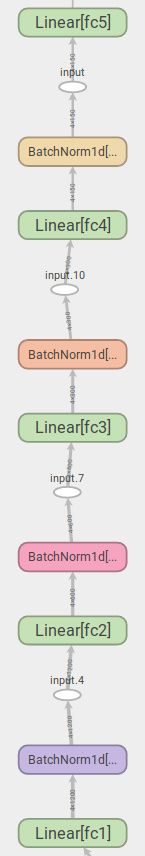
\includegraphics[width=0.5\linewidth]{FFN.jpg}
\caption{\label{fig:FFN} Feed Forward Network Architecture with BatchNorm layers, visualized in TensorBoard.}
\end{figure}
\end{minipage} \hfill
\begin{minipage}{0.6\linewidth}
In order to test the correct implementation of used SSL algorithms, a series of experiments will be performed on the MNIST data set. \cite{lecun-mnisthandwrittendigit-2010}\par 
Originally, the MNIST consists of a training set containing 60000 examples and 10000 examples from the test set. In both cases, the number of examples for each class is equal.\par

As an artificial neural network architecture will be used a simple Feed Forward Network with figure \ref{fig:FFN}.

For the semi-supervised problem, the original dataset will be divided into labeled and un labeled data. On the labelled set, another division into training and validation data will be made. \newline
The images will be standardized with regard to the average and the variance of the whole set, i.e. successively:
    \begin{itemize}
        \item mean: 0.1307
        \item standard deviation: 0.3081
    \end{itemize}
    \newline
Cross entropy will be used as a cost function.
The FixMatch method uses the RandAugment \cite{RandAugment} with the appropriate amount of transformations marked as $N_{weak}$ and their strength $M_{weak}$ and similarly for strong augmentations. Additionally, CutOut \cite{Cutout} was used for strong augmentation.
\The notation that will be used in the resultant tables:
\begin{itemize}
    \item $V$ - validation dataset size
    \item $X_l$ - training labeled dataset size
    \item $X_{unl}$ - training unlabeled dataset size
    \item $T$ - test dataset size
    \item $B$ - labeled batch size
    \item $U$ - unlabeled batch size
\end{itemize}
\end{minipage}
\newpage
The results, together with the selected hyperparameters, are placed in the table \ref{tab:MNIST}.
It may be observed that FixMatch, VAT and pseudolabeeling were the best models respectively, which is consistent with the results of these algorithms in other \cite{Realistic}, \cite{FixMatch} works and may be an argument for a successful implementation of these methods.

\restylefloat{table}

\begin{table*}[p!]
\centering
\resizebox{\textwidth}{!}{ 
\begin{tabular}{@{}rrcrrcrrcrr@{}}\toprule 
& \multicolumn{1}{c}{\textbf{Supervised}} & \phantom{a}
& \multicolumn{1}{c}{\textbf{Pseudo-Label}} & \phantom{a} 
& \multicolumn{1}{c}{\textbf{VAT}} & \phantom{a} 
& \multicolumn{1}{c}{\textbf{FixMatch}}
\\\midrule
\textbf{Hyperparameters:}
\\$X_l$                & 96     &&  96    &&  96    && 96
\\$T$                & 10000  && 10000  && 10000  && 10000
\\$V$                & 960    &&  960   && 960    && 960
\\$B$                & 32     && 32     && 64     && 32     
\\$U$                & -      && 32     && 256    && 224      
\\$Max\;steps$       & 10000  && 10000  && 10000  && 6000    
\\$Initial\;lr$      & 1e-05  && 1e-05  && 2e-05  && 3e-2   
\\$Optimizer$        & Adam   && Adam   && Adam   && SGD
\\$Momentum$         & -      && -      && -      && 0.9   
\\$Weight\;decay$    & -      && -      && -      && 0.0005  
\\$Lr\;scheduler$    & -      && -      && StepLR && LinearWarmupLR 
\\$Decay$ \gamma     & -      && -      && 0.5    && -    
\\$Initial\;decay\;step$& -   && -      && 2000   && -     
\\$Decay\;step\;size$& -      && -      && 2000   && -
\\$Warmup\;steps$    & -      && -      && -      && 1000 
\\$T_1$              & -      && 1      && -      && -
\\$T_2$              & -      && 2000   && -      && - 
\\$Max\;$\lambda      & -      && 1      && -      && - 
\\\lambda             & -      && -      && 1      && - 
\\\varepsilon        & -      && -      && 3     && -  
\\$K$                & -      && -      && 1      && -  
\\\xi                & -      && -      && 1e-06  && -
\\\tau               & -      && -      && -      && 0.999    
\\$N\;weak$          & -      && -      && -      && 1
\\$M\;weak$          & -      && -      && -      && 2
\\$N\;strong$        & -      && -      && -      && 3
\\$M\;strong$        & -      && -      && -      && 5
\\\hline
\\\textbf{Val. Error rate}  & 26.6   && 24.6   && 23.6   && 22.5 
\\\hline
\\\textbf{Test Error rate}  & 24.1   && 21.4   && 20.4   && 18.1
\\\bottomrule
\end{tabular}
}
\caption{Best validation error rates and test error rates for MNIST obtained by Supervised, Pseudo-Label, VAT and FixMatch models with chosen and tuned hyperparameters.}
\label{tab:MNIST}
\end{table*}


\subsection{Experiments in NLP domain} \par

\subsubsection{Components of compared SLL algorithms}
Validated machine learning systems will consist of the following elements:
\begin{itemize}
   \item Processed datasets:
   \begin{itemize}
     \item  IMDB \cite{IMDB}
     \item  MR \cite{MR}
   \end{itemize}
   \item Representation of data:
   \begin{itemize}
     \item  the FastText algorithm was used to represent texts in the form of \textbf{300} dimensional vectors.  \cite{FastText}
   \end{itemize}
   \item Model Architecture:
   \begin{itemize}
     \item   the chosen architecture of the artificial neural network will be the convolution model proposed in \cite{Convolution}. The choice of this architecture is associated with a relatively short processing time of training data, which allows for many experiments. 
     \The hyperparameters associated with the architecture of this model, except for the dropout value, have been chosen arbitrarily and will not change during the process of estimating other algorithm hyperparameters. Their values are:
      \begin{itemize}
      \item number of filters - 32
      \item filter sizes - 1, 2, 3, 5
      \end{itemize}
   \end{itemize}
   \item SSL algorithms:
    \begin{itemize}
    \item the same implementations of SSL methods that were tested during the experiments on the MNIST data set will be used:
        \begin{itemize}
            \item Pseudo-Label
            \item VAT
            \item FixMatch
         \end{itemize}
    \end{itemize}
\end{itemize}



\setlength{\parindent}{4ex}One of the goals of the work is also to see how the FixMatch method works in the NLP domain.
The following text augmentation methods were used to achieve this:
\begin{enumerate}
    \item Weak type augmentation:
        \begin{itemize}
            \item substitute character by keyboard distance
            \item insert character randomly
            \item substitute character randomly
            \item delete char randomly
            \item swap character randomly
            \item insert word by tf-idf similarity
            \item split word into two tokens randomly
            \item swap word randomly
            \item substitute word by it's antonym
            \item substitute word by spelling mistake from special words dictionary
        \end{itemize}
    \item Strong type augmentation: 
        \begin{itemize}
            \item back translation i.e translation of the text from English into French and back into English using the package Tensor2Tensor \cite{tensor2tensor}
        \end{itemize}
\end{enumerate}

\subsubsection{Experiments methodology}
\par The experiments were carried out according to some recommendations from \cite{Realistic}:
\begin{enumerate}
    \item the same type and models's architecture and one code base for all evaluated SSL algorithms 
    \item realistically small validation and training datasets used to select hyperparameters
    \item validation of SSL algorithms with different amount of labeled and unlabeled data
    \item comparison of SSL algorithms to models trained only on labeled data with carefully selected hyperparameters
\end{enumerate}
\par
In the process of hyperparameters selection, \textbf{200} samples from labeled sets and \textbf{400} samples from unlabelled sets were used.
In order to investigate the effect of the ratio of the validation set size to the training set size on the classifier's effectiveness, 3 validation sets of the size of \textbff{40}, \textbff{60}, and \textbf{100} were arbitrarily selected. 
In order to check how a random small sample of the real data set  affects each of the SSL algorithms, training and validation of the model took  place on the \textbf{3} folds with different training and validation data. \par

With the hyperparameters selected, each of the SSL algorithms will be trained on all the available data and will receive a score on a test set for each of the folders. The results obtained in this way will indicate the quality of selected hyperparameters in the validation process and the impact of a random sample of the training set on the variances obtained by the result algorithms.

In order to investigate even more deeply the obtained hyperparameters and the scalability of the SLL algorithms, further experiments will be performed:
    \begin{enumerate}
        \item The algorithms will be trained and tested on the additional amount of tagged and unmagged data simultaneously:
            \begin{itemize}
                \item $D_l = 400, D_{ul} = 800$
                \item $D_l = 600, D_{ul} = 1200$
            \end{itemize}
        \item The algorithms will be trained and tested on additional unlabeled data:
            \begin{itemize}
                    \item $D_l = 200, D_{ul} = 800$
                    \item $D_l = 200, D_{ul} = 1200$
            \end{itemize}
    \end{enumerate}

\subsubsection{Experiments results on IMDB dataset}

\begin{table*}[hp!]
\centering
\resizebox{\textwidth}{!}{  
\begin{tabular}{@{}rrrrcrrrcrrr@{}}
\toprule 
& \multicolumn{3}{c}{\textbf{Pseudo-Label}}
& \phantom{abc}& \multicolumn{3}{c}{\textbf{Supervised}} 
\\\cmidrule{2-4}
\cmidrule{6-8}
\\\textbf{Validation sizes} & $40$ & $60$ & $100$ && $40$ & $60$ & $100$
\\\midrule 
\textbf{Hyperparameters:}
\\$B$                   & 32     & 32     & 32     && 32     & 32     & 32
\\$U$                   & 32     & 32     & 32     && -      & -      & -
\\$Max\;steps$          & 1000   & 1000   & 1000   && 200    & 200    & 200
\\$Initial\;lr$         & 1e-2   & 1e-3   & 1e-3   && 1e-2   & 1e-2   & 1e-2
\\$Dropout$             & 0.1    & 0.2    & 0.1    && 0.2    & 0.2    & 0.1
\\$Optimizer$           & Adam   & Adam   & Adam   && Adam   & Adam   & Adam
\\$T_1$                 & 1      & 1      & 1      && -      & -      & -
\\$T_2$                 & 1000   & 1000   & 1000   && -      & -      & -
\\$Max$ \lambda         & 1      & 1      & 1      && -      & -      & -
\\$Lr\;scheduler$       & StepLR & StepLR & StepLR && StepLR & StepLR & StepLR
\\$Decay\;gamma$        & 0.5    & 0.5    & 0.5    && 0.5    & 0.5    & 0.5
\\$Initial\;decay\;step$& 400    & 200    & 250    && 50     & 50     & 50
\\$Decay\;step\;size$   & 40     & 1      & 1      && 1      & 1      & 1
\\\hline
\\\textbf{Error rate}  & $\SI{37.7\pm0.4}$ & $\SI{42.0\pm6.2}$ & $\SI{42.5\pm6.4}$ && $\SI{41.4\pm12.2}$ & $\SI{37.2\pm1.4}$  & $\SI{39.3\pm1.5}$
\\\bottomrule
\end{tabular}}
\caption{Best validation error rates for IMDB obtained by Supervised and Pseudo-Label models on 3 training folds with tuned hyperparameters on validation datasets with 40, 60 and 100 sample sizes.}
\label{tab:IMDBV1}
\end{table*}

\begin{table*}[hp!]
\centering
\resizebox{\textwidth}{!}{  
\begin{tabular}{@{}rrrrcrrrcrrr@{}}
\toprule 
& \multicolumn{3}{c}{\textbf{FixMatch}}
& \phantom{abc}& \multicolumn{3}{c}{\textbf{VAT}} 
\\\cmidrule{2-4}
\cmidrule{6-8}
\\\textbf{Validation sizes} & $40$ & $60$ & $100$ && $40$ & $60$ & $100$
\\\midrule 
\textbf{Hyperparameters:}
\\$B$                &  32       & 32       & 32       && 64       & 64       & 64
\\$U$                & 224       & 224      & 224      && 256      & 256      & 256
\\$Max\;steps$       & 300       & 300      & 300      && 300      & 300      & 300
\\$Optimizer$        & SGD       & SGD      & SGD      && Adam     & Adam     & Adam
\\$Dropout$          & 0.1       & 0.1      & 0.2      && 0.1      & 0.2      & 0.25
\\$Momentum$         & 0.9       & 0.9      & 0.9      && -        & -        & -
\\$Weight\;decay$    & 0.0005    & 0.0005   & 0.0005   && -        & -        & -
\\$Initial\;lr$      & 3e-2      & 3e-2     & 3e-2     && 2e-5     & 2e-5     & 2e-5
\\$Lr\;scheduler$    & -         & CosineLR & CosineLR && StepLR   & StepLR   & StepLR
\\$Decay\;$\gamma    & -         & -        & -        && 0.5      & 0.5      & 0.5
\\$Initial\;decay\;step$& -         & -        & -        && 20       & 20       & 20
\\$Decay\;step\;size$& -         & -        & -        && 100      & 75       & 80
\\$Warmup\;steps$    & -         & 50       & 50       && -        & -        & -
\\\lambda           & 0.1       & 0.1      & 0.1      && 1        & 1        & 1
\\\varepsilon        & -         & -        & -        && 3        & 3        & 3
\\$K$                & -         & -        & -        && 1        & 1        & 1
\\\xi                & -         & -        & -        && 1e-6     & 1e-6     & 1e-6
\\\tau               & 0.999     & 0.999    & 0.999    && -        & -        & -
\\$N\;weak$          & 1         & 1        & 2        && -        & -        & -
\\\hline
\\\textbf{Error rate}  & $\SI{34.2\pm10.4}$     & $\SI{35.5\pm3.6}$     & $\SI{45.5\pm10.3}$    && $\SI{45.6\pm11.0}$ & $\SI{46.3\pm6.9}$     & $\SI{47.6\pm7.4}$
\\\bottomrule
\end{tabular}}
\caption{Best validation error rates for IMDB obtained by FixMatch and VAT models on 3 training folds with tuned hyperparameters on validation datasets with 40, 60 and 100 sample sizes.}
\label{tab:IMDBV2}
\end{table*}


\begin{table*}[hp!]
\centering
\resizebox{\textwidth}{!}{  
\begin{tabular}{@{}rrrrcrrrcrrr@{}}
\toprule 
& \multicolumn{3}{c}{\textbf{Pseudo-Label}}
& \phantom{abc}& \multicolumn{3}{c}{\textbf{Supervised}} 
\\\cmidrule{2-4}
\cmidrule{6-8}
\\\textbf{Validation sizes} & $40$ & $60$ & $100$ && $40$ & $60$ & $100$
\\\midrule 
\textbf{$\bm{X_l/X_{unl}}$}
\\$200/400$ &$\SI{34.6 \pm 4.0}$ & $\SI{33.6 \pm 3.7}$ & $\SI{28.8 \pm 0.6}$ && $\SI{32.5 \pm 2.2}$ & $\SI{32.5 \pm 0.1}$ & $\SI{32.3 \pm 3.8}$ && 
\\$400/800$ & $\SI{36.7 \pm 4.3}$ & $\SI{31.8 \pm 1.4}$ & $\SI{32.2 \pm 2.8}$ && $\SI{31.0 \pm 1.2}$ & $\SI{30.4 \pm 0.5}$ & $\SI{29.3 \pm 2.5}$ && 
\\$600/1200$ & $\SI{31.2 \pm 0.9}$ & $\SI{32.0 \pm 2.0}$ & $\SI{33.4 \pm 3.9}$ && $\SI{31.2 \pm 0.9}$ & $\SI{32.0 \pm 2.0}$ & $\SI{33.4 \pm 3.9}$ && 
\\$200/800$ & $\SI{33.9 \pm 1.1}$ & $\SI{32.9 \pm 3.0}$ & $\SI{33.3 \pm 4.3}$ && - & - & - && 
\\$200/1200$ & $\SI{33.9 \pm 1.1}$ & $\SI{32.8 \pm 3.0}$ & $\SI{33.3 \pm 4.3}$ && - & - & - && 
\\\bottomrule
\end{tabular}}
\caption{Test error rates for IMDB obtained by Pseudo-Label and Supervised models on 3 training folds(with different labeled and unlabeled sample sizes). Hyperparameters for those models were tuned using 200 labeled and 400 unlabeled training samples on validation datasets with 40, 60 and 100 sample sizes.}
\label{tab:IMDBT1}
\end{table*}

\begin{table*}[hp!]
\centering
\resizebox{\textwidth}{!}{  
\begin{tabular}{@{}rrrrcrrrcrrr@{}}
\toprule 
& \multicolumn{3}{c}{\textbf{FixMatch}}
& \phantom{abc}& \multicolumn{3}{c}{\textbf{VAT}} 
\\\cmidrule{2-4}
\cmidrule{6-8}
\\\textbf{Validation sizes} & $40$ & $60$ & $100$ && $40$ & $60$ & $100$
\\\midrule 
\textbf{$\bm{X_l/X_{unl}}$}
\\$200/400$ &$\SI{50.9 \pm 2.2}$ & $\SI{46.8 \pm 4.3}$ & $\SI{47.1 \pm 3.3}$ && $\SI{41.0 \pm 1.5}$ & $\SI{42.6 \pm 1.8}$ & $\SI{42.3 \pm 1.7}$ && 
\\$400/800$ & $\SI{50.9 \pm 2.6}$ & $\SI{46.1 \pm 3.8}$ & $\SI{46.7 \pm 2.7}$ && $\SI{41.0 \pm 1.9}$ & $\SI{37.0 \pm 2.0}$ & $\SI{40.2 \pm 3.6}$ && 
\\$600/1200$ & $\SI{49.8 \pm 1.5}$ & $\SI{46.3 \pm 5.5}$ & $\SI{47.6 \pm 2.9}$ && $\SI{40.7 \pm 0.5}$ & $\SI{37.5 \pm 0.1}$ & $\SI{41.5 \pm 1.1}$ && 
\\$200/800$ & $\SI{50.8 \pm 1.9}$ & $\SI{50.4 \pm 1.9}$ & $\SI{47.4 \pm 2.8}$ && $\SI{41.0 \pm 1.3}$ & $\SI{41.3 \pm 2.0}$ & $\SI{42.3 \pm 1.7}$ && 
\\$200/1200$ & $\SI{48.5 \pm 6.4}$ & $\SI{50.3 \pm 1.6}$ & $\SI{47.1 \pm 3.3}$ && $\SI{41.0 \pm 1.4}$ & $\SI{41.3 \pm 2.0}$ & $\SI{43.2 \pm 1.7}$ && 
\\\bottomrule
\end{tabular}}
\caption{Test error rates for IMDB obtained by FixMatch and VAT models on 3 training folds(with different labeled and unlabeled sample sizes). Hyperparameters for those models were tuned using 200 labeled and 400 unlabeled training samples on validation datasets with 40, 60 and 100 sample sizes.}
\label{tab:IMDBT2}
\end{table*}

\begin{table*}[hp!]
\centering
\resizebox{\textwidth}{!}{  
\begin{tabular}{@{}rrrrcrrrcrrr@{}}
\toprule 
& \multicolumn{3}{c}{\textbf{Pseudo-Label}}
& \phantom{abc}& \multicolumn{3}{c}{\textbf{Supervised}} 
\\\cmidrule{2-4} \cmidrule{6-8}
\\\textbf{Validation sizes} & $40$ & $60$ & $100$ && $40$ & $60$ & $100$
\\\midrule 
\textbf{Hyperparameters:}
\\$B$   & 32     & 32     & 32     && 32     & 32     & 32
\\$U$ & 32     & 32     & 32     && -      & -      & -
\\$Max\;steps$       & 200    & 1000   & 200    && 200    & 200    & 200
\\$Initial\;lr$      & 1e-2   & 1e-1   & 1e-1   && 1e-3   & 1e-2   & 1e-2
\\$Dropout$          & 0.1    & 0.1    & 0.2    && 0.1    & 0.1    & 0.3
\\$Optimizer$        & Adam   & Adam   & Adam   && Adam   & Adam   & Adam
\\$T_1$              & 1    & 1    & 1    && -      & -      & -
\\$T_2$              & 200    & 200    & 200    && -      & -      & -
\\$Max\;$\lambda  & 1  & 1      & 1      && -      & -      & -
\\$Lr\;scheduler$    & StepLR & -      & StepLR && -      & -      & -
\\$Decay\;$\gamma      & 0.5    & -      & 0.5    && -      & -      & -
\\$Initial\;decay\;step$       & 400    & -      & 60     && -      & -      & -
\\$Decay\;step\;size$  & 40     & -      & 20     && -      & -      & -
\\\hline
\\\textbf{Error rate}  & $\SI{25.0\pm6.2}$   & $\SI{34.1\pm6.2}$   & $\SI{37.8\pm2.5}$   && $\SI{42.3\pm1.2}$  & $\SI{42.1\pm4.8}$    & $\SI{45.2\pm3.1}$
\\\bottomrule
\end{tabular}}
\caption{Best validation error rates for MR obtained by Supervised and Pseudo-Label models on 3 training folds with tuned hyperparameters on validation datasets with 40, 60 and 100 sample sizes.}
\label{tab:MRV1}
\end{table*}

\begin{table*}[hp!]
\centering
\resizebox{\textwidth}{!}{  
\begin{tabular}{@{}rrrrcrrrcrrr@{}}
\toprule 
& \multicolumn{3}{c}{\textbf{FixMatch}}
& \phantom{abc}& \multicolumn{3}{c}{\textbf{VAT}} 
\\\cmidrule{2-4}
\cmidrule{6-8}
\\\textbf{Validation sizes} & $40$ & $60$ & $100$ && $40$ & $60$ & $100$
\\\midrule 
\textbf{Hyperparameters:}
\\$B$                &  32       & 32       & 32       && 64       & 64       & 64
\\$U$                & 224       & 224      & 224      && 256      & 256      & 256
\\$Max\;steps$       & 300       & 300      & 300      && 300      & 600      & 600
\\$Dropout$          & 0.1       & 0.1      & 0.1      && 0.1      & 0.2      & 0.2
\\$Optimizer$        & SGD       & SGD      & SGD      && Adam     & Adam     & Adam
\\$Momentum$         & 0.9       & 0.9      & 0.9      && -        & -        & -
\\$Weight\;decay$    & 5e-4      & 5e-4     & 1e-3     && -        & -        & -
\\$Initial\;lr$      & 3e-2      & 3e-2     & 3e-2     && 2e-5     & 2e-5     & 2e-5
\\$Lr\;scheduler$    & -         & CosineLR & CosineLR && -        & StepLR   & StepLR
\\$Decay\;$\gamma    & -         & -        & -        && -        & 0.5      & 0.5
\\$Initial\;decay\;step$& -         & -        & -        && -        & 50       & 20
\\$Decay\;step\;size$& -         & -        & -        && -        & 200      & 180
\\$Warmup\;steps$    & -         & 50       & 50       && -        & -        & -
\\\lambda            & 0.1       & 0.1      & 0.1      && 1        & 1        & 1
\\\epsilon           & -         & -        & -        && 3        & 3        & 3
\\$K$                & -         & -        & -        && 1        & 1        & 1
\\\xi                & -         & -        & -        && 1e-6     & 1e-6     & 1e-6
\\\tau               & 0.999     & 0.999    & 0.999    && -        & -        & -
\\$N\;weak$          & 1         & 2        & 2        && -        & -        & -
\\\hline
\\\textbf{Error rate}  & $\SI{46.3\pm3.8}$ & $\SI{47.2 \pm6.0}$ & $\SI{44.9 \pm4.4}$    && $\SI{41.4 \pm19.1}$ & $\SI{45.6 \pm10.0}$     & $\SI{46.4 \pm10.3}$
\\\bottomrule
\end{tabular}}
\caption{Best validation error rates for MR obtained by FixMatch and VAT models on 3 training folds with tuned hyperparameters on validation datasets with 40, 60 and 100 sample sizes.}
\label{tab:MRV2}
\end{table*}

\begin{table*}[hp!]
\centering
\resizebox{\textwidth}{!}{  
\begin{tabular}{@{}rrrrcrrrcrrr@{}}
\toprule 
& \multicolumn{3}{c}{\textbf{Pseudo-Label}}
& \phantom{abc}& \multicolumn{3}{c}{\textbf{Supervised}} 
\\\cmidrule{2-4}
\cmidrule{6-8}
\\\textbf{Validation sizes} & $40$ & $60$ & $100$ && $40$ & $60$ & $100$
\\\midrule 
\textbf{$\bm{X_l/X_{unl}}$}
\\$200/400$ &$\SI{44.5 \pm 3.4}$ & $\SI{48.0 \pm 2.6}$ & $\SI{44.0 \pm 3.6}$ && $\SI{44.2 \pm 4.6}$ & $\SI{44.2 \pm 5.9}$ & $\SI{43.2 \pm 4.6}$ && 
\\$400/800$ & $\SI{42.6 \pm 1.3}$ & $\SI{41.3 \pm 3.3}$ & $\SI{41.2 \pm 2.7}$ && $\SI{43.9 \pm 4.3}$ & $\SI{41.8 \pm 3.8}$ & $\SI{40.5 \pm 1.3}$ && 
\\$600/1200$ & $\SI{41.6 \pm 2.3}$ & $\SI{41.9 \pm 1.2}$ & $\SI{38.4 \pm 0.4}$ && $\SI{39.4 \pm 2.4}$ & $\SI{43.5 \pm 7.2}$ & $\SI{38.1 \pm 2.7}$ && 
\\$200/800$ & $\SI{44.5 \pm 3.4}$ & $\SI{47.2 \pm 3.8}$ & $\SI{44.0 \pm 3.6}$ && - & - & - && 
\\$200/1200$ & $\SI{44.2 \pm 3.9}$ & $\SI{47.2 \pm 3.8}$ & $\SI{44.0 \pm 3.6}$ && - & - & - && 
\\\bottomrule
\end{tabular}}
\caption{Test error rates for MR obtained by Pseudo-Label and Supervised models on 3 training folds(with different labeled and unlabeled sample sizes). Hyperparameters for those models were tuned using 200 labeled and 400 unlabeled training samples on validation datasets with 40, 60 and 100 sample sizes.}
\label{tab:MRT1}
\end{table*}

\begin{table*}[hp!]
\centering
\resizebox{\textwidth}{!}{  
\begin{tabular}{@{}rrrrcrrrcrrr@{}}
\toprule 
& \multicolumn{3}{c}{\textbf{FixMatch}}
& \phantom{abc}& \multicolumn{3}{c}{\textbf{VAT}} 
\\\cmidrule{2-4}
\cmidrule{6-8}
\\\textbf{Validation sizes} & $40$ & $60$ & $100$ && $40$ & $60$ & $100$
\\\midrule 
\textbf{$\bm{X_l/X_{unl}}$}
\\$200/400$ &$\SI{47.7 \pm 2.4}$ & $\SI{48.7 \pm 2.8}$ & $\SI{46.3 \pm 4.8}$ && $\SI{42.9 \pm 4.4}$ & $\SI{43.4 \pm 3.8}$ & $\SI{43.7 \pm 33.3}$ && 
\\$400/800$ & $\SI{47.9 \pm 8.2}$ & $\SI{49.6 \pm 1.2}$ & $\SI{50.4 \pm 1.2}$ && $\SI{39.7 \pm 3.6}$ & $\SI{45.4 \pm 1.7}$ & $\SI{42.1 \pm 4.2}$ && 
\\$600/1200$ & $\SI{48.4 \pm 6.6}$ & $\SI{48.8 \pm 0.7}$ & $\SI{50.0 \pm 2.2}$ && $\SI{38.4 \pm 5.3}$ & $\SI{31.2 \pm 1.3}$ & $\SI{33.3 \pm 4.3}$ && 
\\$200/800$ & $\SI{50.6 \pm 8.6}$ & $\SI{51.9 \pm 9.1}$ & $\SI{47.6 \pm 3.0}$ && $\SI{45.1 \pm 1.9}$ & $\SI{45.1 \pm 1.7}$ & $\SI{44.0 \pm 2.8}$ && 
\\$200/1200$ & $\SI{47.1 \pm 8.4}$ & $\SI{51.4 \pm 8.7}$ & $\SI{48.5 \pm 2.8}$ && $\SI{46.1 \pm 1.3}$ & $\SI{45.6 \pm 2.0}$ & $\SI{43.9 \pm 2.7}$ && 
\\\bottomrule
\end{tabular}}
\caption{Test error rates for MR obtained by FixMatch and VAT models on 3 training folds(with different labeled and unlabeled sample sizes). Hyperparameters for those models were tuned using 200 labeled and 400 unlabeled training samples on validation datasets with 40, 60 and 100 sample sizes.}
\label{tab:MRT2}
\end{table*}

\paragraph{Hyperparameter estimation}
\par Table no.\ref{tab:IMDBV1} shows hyperparameters and the best results are visible on the different validation sets for 3 folders with different training and validation data for Pseudo-Label and Supervised algorithms.
\begin{itemize}
    \item Pseudo-Label:
    \begin{itemize}
          \item the lowest average and variance error rate was obtained by a model validated on 40 samples.
          \itme the largest average and variance error rate was obtained with a model validated on 100 samples.
    \end{itemize}
    \I'm Supervised:
    \begin{itemize}
        \item the lowest average and error rate variances were obtained by a model validated on 60 samples.
        \item the largest average and error rate variance was obtained with a model validated on 40 samples.
    \end{itemize}
\end{itemize}


\par Table no. \ref{tab:IMDBV2} shows hyperparameters and the best results on the different validation sets for 3 folds with different training and validation data for FixMatch and VAT algorithms.
\begin{itemize}
    \item FixMatch:
    \begin{itemize}
        \item the smallest average error rate and the largest variance of the error rate was obtained by a model validated on 40 samples.
        \item the smallest variance of the error rate was obtained with a model validated on 60 samples.
        \item the largest average error rate was obtained with a model validated on 100 samples.
    \end{itemize}
    \VAT:
    \begin{itemize}
        \item the same results as for FixMatch
    \end{itemize}
\end{itemize}
\vspace{5mm} %5mm vertical space
\vspace{5mm} %5mm vertical space
\paragraph{Results on test datasets}
In table no. \ref{tab:IMDBT1} it can be observed:
\begin{itemize}
    \item for Pseudo-Label models
    \begin{itemize}
        \item that among the models validated on 40 samples the smallest average error was obtained by the model with the ratio of the number of labeled data to the number of unlabeled data equal to 600 /1200. The same model on the validation set obtained the smallest average error and the smallest variance. Adding new labelled and unlabeled data reduces the average error rate. 
        
        \item that among the models validated on 100 samples, the smallest average error had a model with the ratio of labelled to unlabeled data equal to 200/400. The same model on the validation set obtained the largest average error rate and the largest variance error rate. The model has a relatively low error, but the results do not scale with the new data, it seems that the new data spoil the effectiveness of the model.
        
    \end{itemize}
    \item for Supervised models
    \begin{itemize}
        \item that among the models validated on 40 samples the smallest average error was obtained in the model with the ratio of the number of labelled to unlabelled data equal to 400/800. The same model on the validation set obtained the largest average and error rate variance. Adding new labelled and unlabeled data does not reduce the average error rate. 
        
        \item that among the models validated on 60 samples the smallest average error was obtained by the model with the ratio of the number of tagged data to the number of unlabeled data equal to 400/800. The same model on the validation set obtained the smallest average error and the smallest variance. Adding new labeled and unlabeled data does not reduce the average error rate. 
    \end{itemize}
\end{itemize}
\vspace{5mm} %5mm vertical spa
The following conclusions can be drawn from the above observations:
    \begin{itemize}
        \item in the case of the Pseudo-Label algorithm, it turns out that in order to choose the model that best classifies on the test set, it would be completely non-intuitive to choose the model with the greatest variance and the greatest error on the validation set. The results obtained by the algorithm are lower than those for supervised baseline except for one model. It can be assumed that too little validation data was used and/or the algorithm was trained with too few steps to estimate the correct hyperparameters for efficient classification with less error rate score than supervised baseline.
        \item in the case of supvervised baseline, the choice of the model taking into account the average error or its variance on the validation set does not affect the results on the test set to be significantly better.
    \end{itemize}

\vspace{5mm} %5mm vertical space
\vspace{5mm} %5mm vertical space
In table no. \ref{tab:IMDBT2} it can be observed:
\begin{itemize}
    \item for FixMatch models:
    \begin{itemize}
        \item that among the models validated on 40 samples the smallest average error was obtained by the model with the ratio of the number of labeled data to the number of unlabeled data equal to 200/1200. The same model on the validation set obtained the smallest average error and the largest variance. This model basically makes random decisions with an error close to 50. Addition of new labeled and unlabeled data does not reduce the average error rate. 
         \item that among the models validated on 60 samples the smallest average error was obtained by the model with the ratio of the number of labeled data to the number of unlabeled data  equal to 400 to 800. The same model, on the validation set, obtained the smallest variance of error. This model basically makes random decisions when the error is close to 50.
         Adding new tagged and unlabeled data does not reduce the average error rate.  
        \item that among the models validated on 100 samples the smallest average error had a model with the ratio of the number of labeled data to the number of unlabeled data equal to 400/800 the same model on the validation set obtained the largest average error.  As with the rest of the models for the FixMatch algorithm, the average error rate does not change after adding labeled or unlabelled data.  
    \end{itemize}
    \item for VAT models
    \begin{itemize}
        \item that among the models validated on 40 samples the smallest average error was obtained by the model with the ratio of the number of labeled data to the number of unlabeled data equal to 600/1200. The same model on the validation set has the smallest average error rate. The model will yield slightly better results for more labeled and unlabeled data.
        \item that among the models validated on 60 samples the smallest average error was obtained by the model with the ratio of the number of labeled data to the number of unlabeled data equal to 400/800. The same model on the validation set obtained the smallest variance. The model gets much better effects with the increase of tagged and unlabeled data, and slightly better with the increase of unlabeled data.
        \item that among the models validated on 100 samples the smallest average error was obtained by the model with the ratio of the number of labeled data to the number of unlabeled data equal to 400/800. The same model on the validation set has obtained the largest average error. Adding new labeled and unlabeled data does not reduce the average error rate. 
    \end{itemize}
\end{itemize}
\vspace{5mm} %5mm vertical spa
The following conclusions can be drawn from the above observations:
    \begin{itemize}
        \item in the case of the FixMatch algorithm, the best generalizing factor on the test set is the smallest error rate variance on the validation set. It can be assumed that too little validation data was used for FixMatch and/or the algorithm was trained with too few steps to estimate the right hyperparameters to make the correct classification with less error rate than supervised baseline.
        \item in case of the VAT algorithm, the smallest error variance on the validation set translates into results on the test set. The trade off between the amount of validation and training data which equal to 60 validation samples proved to be optimal, but the effectiveness of the model is still much lower than for the supervised model. It can be assumed that an increase in the number of training steps would result in a better result on the test set.
    \end{itemize}
\subsubsection{Experiments results on MR dataset}

\paragraph{Hyperparameter estimation} 
\par The table no. \ref{tab:MRV1} shows hyperparameters and the best results on the different validation sets for 3 folds (with different training and validation data) for Pseudo-Label and Supervised algorithms.
\begin{itemize}
   \item Pseudo-Label:
    \begin{itemize}
        \item the smallest average error rate and the largest variance of the error rate was obtained by a model validated on 40 samples.
        \item the largest average error rate and the smallest variance was obtained with a model validated on 100 samples.
    \end{itemize}
    \item Supervised:
    \begin{itemize}
        \item the smallest average error rate and the largest variance of the error rate was obtained by a model validated on 60 samples.
        \item the largest average error rate was obtained with a model validated on 100 samples.
        \item the smallest variance of the error rate was obtained with a model validated on 40 samples.
    \end{itemize}
\end{itemize}

\par Table no. \ref{tab:MRV2} shows hyperparameters and the best results on the different validation sets for 3 folds (with different training and validation data) for FixMatch and VAT algorithms.
\begin{itemize}
    \item FixMatch:
    \begin{itemize}
        \item the smallest average error rate was obtained with a model validated on 100 samples.
        \item the smallest variant error rate obtained a model validated on 40 samples.
        \item the largest average error rate and its variant received a model validated on 60 samples.
    \end{itemize}
    \item VAT:
    \begin{itemize}
        \item the largest average error rate was obtained with a model validated on 100 samples.
        \item the smallest variance of the error rate was obtained with a model validated on 60 samples.
        \item the smallest average error rate and the largest variant of the error rate was obtained with a model validated on 40 samples.
    \end{itemize}
\end{itemize}
\vspace{5mm} %5mm vertical space
\vspace{5mm} %5mm vertical space
\paragraph{Results on test datasets}
In table no. \ref{tab:MRT1} it  can be observed
\begin{itemize}
    \item for Pseudo-Label models
    \begin{itemize}
        \item that among the models validated on 40 samples the smallest average error was obtained by the model with the ratio of the number of labeled data to the number of unlabeled data equal to 600/1200. The same model on the validation set obtained the smallest average pale and the largest variance. The average error decreases with the addition of labeled and unlabeled data. 
        \item that among the models validated on 100 samples the smallest average error was obtained by the model with the ratio of the number of labeled data to the number of unlabeled data equal to 400/800. The same model on the validation set obtained the largest average error rate and the smallest variance error rate. The average error decreases with the addition of labeled and unlabeled data.
    \end{itemize}
    \item for Supervised models
    \begin{itemize}
        \item that among the models validated on 40 samples the smallest average error was obtained by the model with the ratio of the number of labeled data to the number of unlabeled data equal to 600/1200. The same model on the validation set obtained the largest average and error rate variance. The average error rate decreases with the addition of new labeled and unlabeled data.  
        \item that among the models validated on 60 samples the smallest average error was obtained by the model with the ratio of the number of labeled data to the number of unlabeled data equal to 400/800. The same model on the validation set obtained the smallest average error and the largest variance. The average pale does not decrease with the addition of labelled and unlabeled data. 
        \item that among the models validated on 100 samples the smallest average error was obtained by the model with the ratio of the number of labeled data to the number of unlabeled data equal to 600/1200. The same model on the validation set has obtained the largest average error. The average error decreases with the addition of labeled and unlabeled data.  
    \end{itemize}
\end{itemize}
\vspace{5mm} %5mm vertical spa
The following conclusions can be drawn from the above observations:
    \begin{itemize}
        \item in the case of the Pseudo-Label algorithm, it turns out that not the average error result on the validation set but it's variance is a good indicator of successful model generalization on the test set. The results obtained by the model are lower than those for supervised baseline. It can be assumed that too little validation data was used and/or the algorithm was trained with too few steps to estimate the correct hyperparameters for correct classification with  error rate smaller than supervised baseline.
        \item in the case of supervised baseline, similarly as in the Pseudo-Label algorithm, not an average but the variance of the error rates is a good indicator of the quality of the models' results on the test set. 
    \end{itemize}
\newline
\vspace{5mm} %5mm vertical space
\vspace{5mm} %5mm vertical space
In table no. \ref{tab:MRT2} it can be observed:
\begin{itemize}
    \item for FixMatch models:
    \begin{itemize}
        \item that among the models validated on 40 samples the smallest average error was obtained by the model with the ratio of the number of labeled data to the number of unlabeled data equal to 200/1200. The same model on the validation set has obtained the smallest average error. The average error does not decrease with the addition of labeled and unlabeled data.
         \item that among the models validated on 60 samples the smallest average error was obtained by the model with the ratio of the number of labeled data to the number of unlabeled data equal to 600/1200. The same model on the validation set obtained the largest average error and the largest variance of error.  The average error does not decrease with the addition of labeled and unlabeled data. 
        \item that among the models validated on 100 samples the smallest average error was obtained by the model with the ratio of the number of labeled data to the number of unlabeled data equal to 200/400. The same model on the validation set has obtained the smallest average error. The average error does not decrease with the addition of labeled and unlabeled data.
    \end{itemize}
    \item for VAT models:
    \begin{itemize}
        \item that among the models validated on 40 samples the smallest average error was obtained by the model with the ratio of the number of labeled data to the number of unlabeled data equal to 600/1200. The same model on the validation set obtained the smallest average and the largest error rate variance. The average error rate decreases with the addition of labeled data.
        \item that among the models validated on 60 samples the smallest average error was obtained by the model with the ratio of the number of labeled data to the number of unlabeled data equal to 400/800. The same model on the validation set obtained the smallest variance. The average error decreases with the addition of labeled data. The model obtains smaller average error than supervised baseline.
        \item that among the models validated on 100 samples the smallest average error was obtained by the model with the ratio of the number of labeled data to the number of unlabeled data equal to 400/800. The same model on the validation set has obtained the largest average error. The average error decreases with the addition of labeled data. 
    \end{itemize}
\end{itemize}
\vspace{5mm} %5mm vertical spa
The following conclusions can be drawn from the above observations:
    \begin{itemize}
        \item for the FixMatch algorithm, the average error on the validation set translates into results on the test set. It can be assumed that too little validation data was used for FixMatch and/or the algorithm was trained with too few steps to estimate the right hyperparameters to make the correct classification with less error rate than supervised baseline.
        \item in case of the VAT algorithm, the smallest error variance on the validation set translates into results on the test set. One of the trained models achieved a smaller error than supervised baseline. It can be assumed that too few steps were used to teach the model and/or too few validation examples were used to correctly select the hyperparameters that will give the model better classification results as the unlabeled number of samples increase.
    \end{itemize}

\section{Conclusions and Future Works}
It was not possible to train a FixMatch model that would have been more effective than the Pseudo-Labeling and VAT method, and even supervised baseline on the used amount of training and validation data. It can be hypothesized that the number of validation data and/or the duration of the algorithm training was too low.
Depending on the used SSL algorithm, the variance or average error on the folds are the parameters that should considered when choosing the best hyperparameters. In most cases better results on the test set were given by models trained and validated on the validation set of size 60 and 100, so it can be hypothesized that it is worth to use slightly less or equal number of ratio between the validation data samples to training data samples, in case of small amount of labelled data.
Most of the VAT and PS models have scaled up as the amount of labelled data increases.
Only the VAT method from the tested SSL methods used on the MR set proved to be better than the supervised baseline for any amount of the proposed validation data. On this basis it can be hypothesized that it is a method that works well with a very small amount of training and validation data.
In order to improve the result of the FixMatch algorithm and other SSL methods, it would be necessary to increase the number of steps and perform experiments on larger amounts of labelled and unlabeled data. Such experiments will be future work that should be done in order to analyze more thoroughly the discussed SSL methods.

\medskip

\bibliographystyle{unsrt}
\bibliography{literature_all}

\end{document}
